%%% LaTeX Template: Two column article
%%%
%%% Source: http://www.howtotex.com/
%%% Feel free to distribute this template, but please keep to referal to http://www.howtotex.com/ here.
%%% Date: February 2011

%%% Preamble
\documentclass[	DIV=calc,%
							paper=a4,%
							fontsize=11pt,%
							twocolumn]{scrartcl}	 					% KOMA-article class

\usepackage[backend=bibtex]{biblatex}         % Citations
\bibliography{main}

\usepackage[english]{babel}										% English language/hyphenation
\usepackage[protrusion=true,expansion=true]{microtype}				% Better typography
\usepackage[pdftex]{graphicx}									% Enable pdflatex
\usepackage[svgnames]{xcolor}									% Enabling colors by their 'svgnames'
\usepackage[hang, small,labelfont=bf,up,textfont=it,up]{caption}	% Custom captions under/above floats
\usepackage{pdfpages}
\usepackage{fix-cm}													  % Custom fontsizes
\usepackage[utf8]{inputenc}                   % Unicode input
\usepackage{tcolorbox}
\usepackage{enumitem}
\usepackage[colorinlistoftodos,prependcaption,textsize=tiny]{todonotes}

%%% Custom sectioning (sectsty package)
\usepackage{sectsty}													% Custom sectioning (see below)
\allsectionsfont{%															% Change font of al section commands
	\usefont{OT1}{phv}{b}{n}%										% bch-b-n: CharterBT-Bold font
	}

\sectionfont{%																% Change font of \section command
	\usefont{OT1}{phv}{b}{n}%										% bch-b-n: CharterBT-Bold font
	}

% custom framed box

\newtcolorbox{framefloat}[1][!tb]{arc=0pt,outer arc=0pt,boxrule=0.4pt,
  colframe=black,colback=white,float=#1}


%%% Headers and footers
\usepackage{fancyhdr}												% Needed to define custom headers/footers
	\pagestyle{fancy}														% Enabling the custom headers/footers
\usepackage{lastpage}

% Header (empty)
\lhead{}
\chead{}
\rhead{}
% Footer (you may change this to your own needs)
\lfoot{\footnotesize Exploratory data analysis for the digital humanities: the Comédie Française Registers Project}
\cfoot{}
\rfoot{\footnotesize page \thepage\ of \pageref{LastPage}}	% "Page 1 of 2"
\renewcommand{\headrulewidth}{0.0pt}
\renewcommand{\footrulewidth}{0.4pt}


\bibliography{main}


%%% Title, author and date metadata
\usepackage{titling}															% For custom titles

\newcommand{\HorRule}{\color{DarkGoldenrod}%			% Creating a horizontal rule
									  	\rule{\linewidth}{1pt}%
										}
%%begin novalidate
\pretitle{\vspace{-30pt} \begin{flushleft} \HorRule
				\fontsize{30}{30} \usefont{OT1}{phv}{b}{n} \color{DarkRed} \selectfont
				}
\title{Exploratory data analysis for the digital humanities}					% Title of your article goes here
\posttitle{\end{flushleft}\vskip 0.5em}

\preauthor{\begin{flushleft}
					\large \lineskip 0.5em \usefont{OT1}{phv}{b}{sl} \color{DarkRed}}
\author{Christopher York, }										% Author name goes here
\postauthor{\footnotesize \usefont{OT1}{phv}{m}{sl} \color{Black}
          Yale University \& MIT Hyperstudio
					\thanks{Many thanks to Elyse Graham for editorial guidance and concluding suggestions.}
					\end{flushleft}
	\HorRule
	\newline
	\footnotesize
In 2008 the Comédie Française, France's pre-eminent dramatic troupe and theater, embarked on an ambitious project to digitize its remarkable collection of ticket receipts dating from the theater's opening in 1680 to just after the French Revolution.  This paper describes the design and development of a general-purpose online data analytics tool to make meaning from the resulting database: its technical and theoretical underpinnings, its audience and constraints, user-base and expectations.
	\HorRule}
%%end novalidate
\date{}																				% No date

%%% Begin document
\begin{document}
\maketitle
\thispagestyle{fancy} 			% Enabling the custom headers/footers for the first page

\subsection*{The Comédie Française Registers Project}

In 2008 the Comédie Française, France's pre-eminent dramatic troupe and theater, embarked on an ambitious project to digitize its remarkable collection of ticket receipts dating from the theater's opening in 1680 to just after the French Revolution.  This paper describes the design and development of a general-purpose online data analytics tool to make meaning from the resulting database: its technical and theoretical underpinnings, its audience and constraints, user-base and expectations.

\begin{figure}
  \centering
  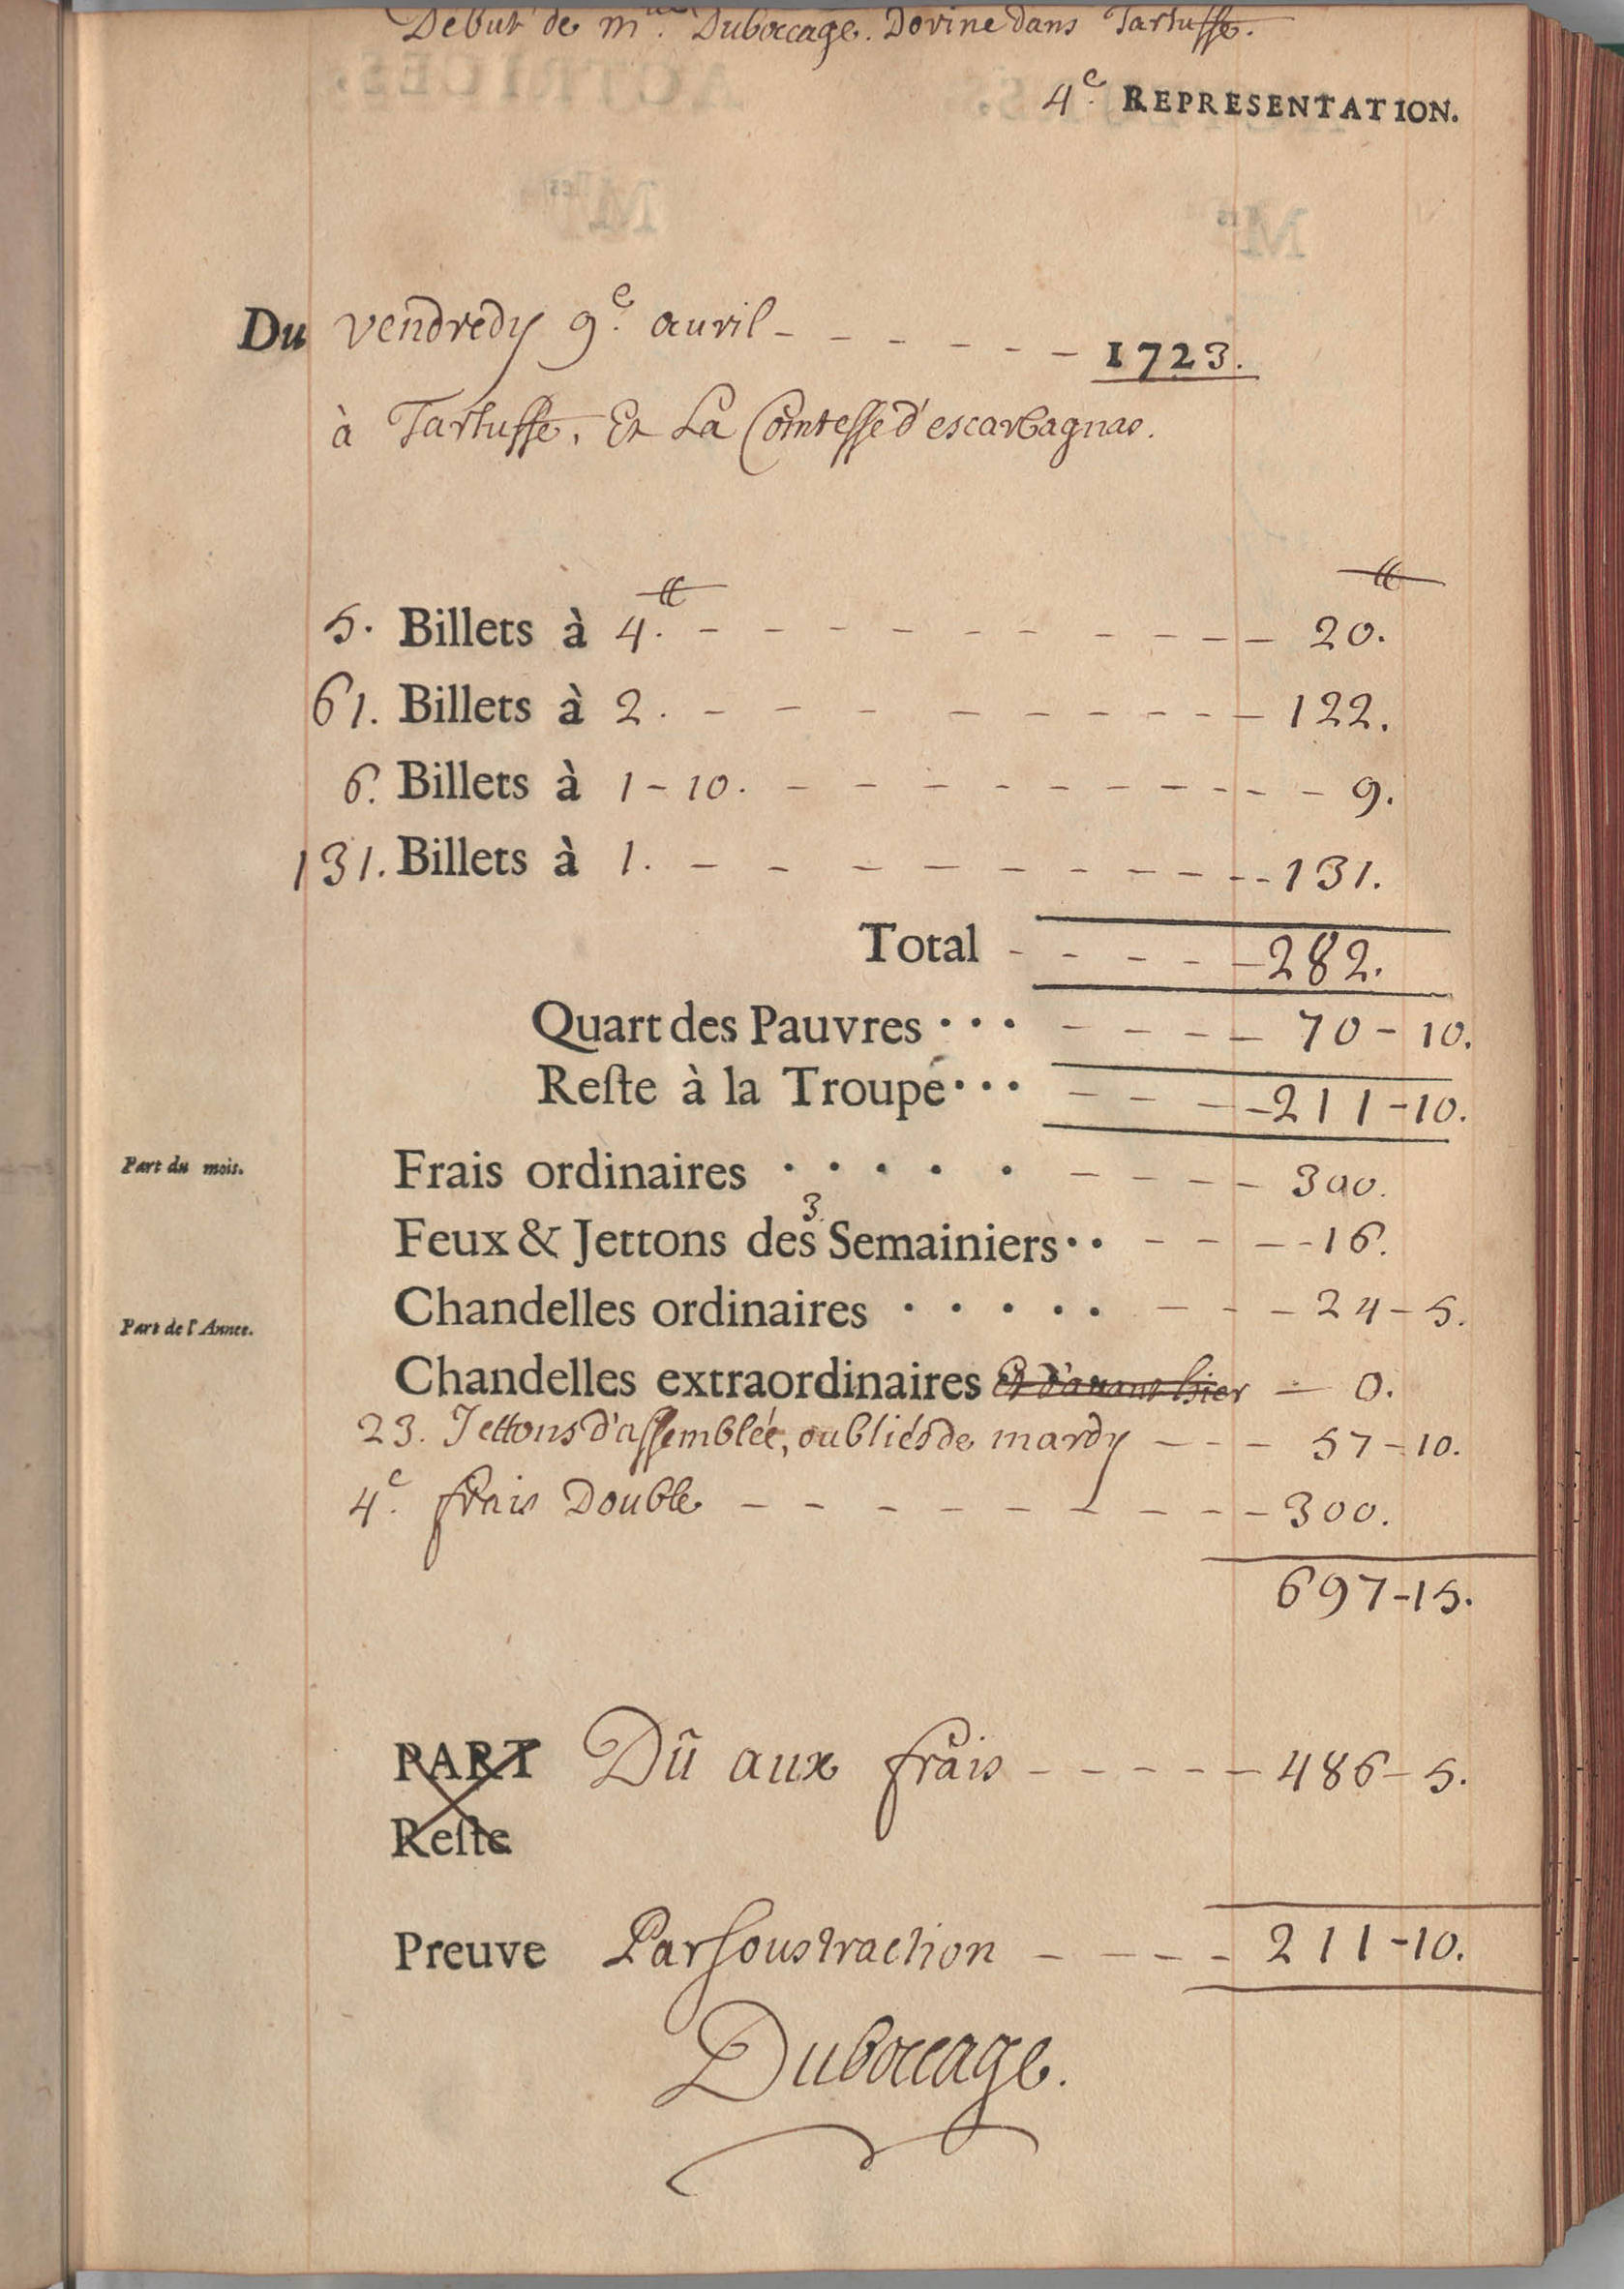
\includegraphics[width=2.5in]{steps/register-example.jpg}
	\caption{A register page from the Comédie Française.}
  \label{fig:register_example}
  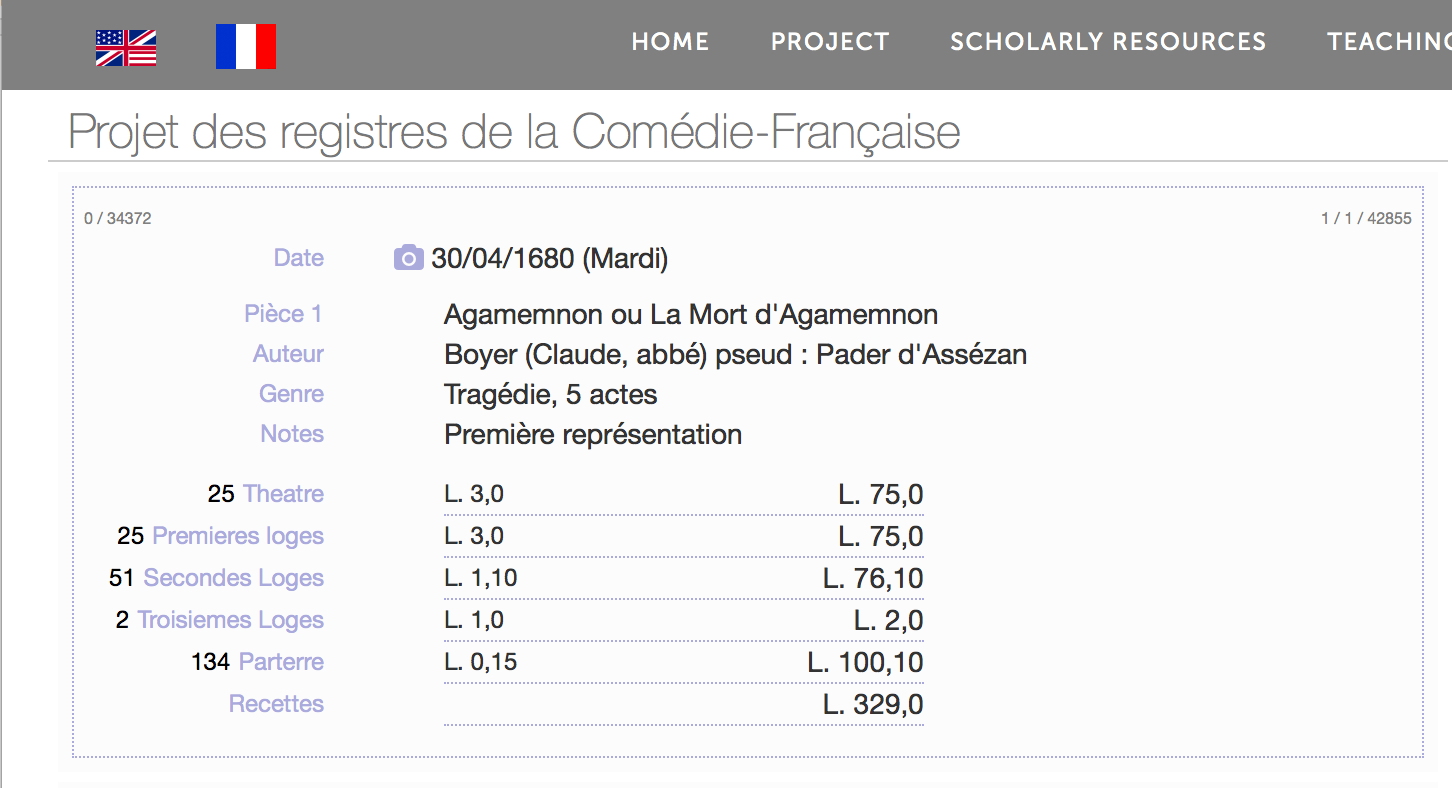
\includegraphics[width=3in]{steps/register-example-digital.png}
	\caption{The corresponding CFRP database record.}
  \label{fig:register_example_digital}
\end{figure}

The Comédie Française had exclusive rights to perform works by Molière, Corneille, Racine, Voltaire, Beaumarchais and other French-language playwrights through an era of critical change in Early Modern France.  Consequently, its archives provide a unique lens into the development of both French theater and French society.  In its daily registers, a member of the troupe recorded the date, bill of plays performed, and itemized how many tickets sold at each price.  This information forms the core of the Comédie Française Registers Project dataset (see figures \ref{fig:register_example} and \ref{fig:register_example_digital}), and is immediately suggestive to readers with dramatic or historical interests.  Using it, one could trace the growth and popularity -- on a daily, play-by-play basis -- of the authors who came to constitute the French literary canon.  Much more ambitiously, the presence of receipts amounts and numbers suggests one could paint a picture of the audience: its demography, temperament, and changing political concerns.

How did certain authors and plays become central to French thought and identity?  Did the popularity of Molière, Racine and Corneille wane as new authors enjoyed a wave of popularity begining in 1740?  Who went to the theater in Early Modern France: soldiers, aristocrats, laborers, women, royalty, merchants?  How did members of these groups afford their entertainment, and how did those economic dynamics affect institutional decisions made by the Comédie Française?  While data from the registers cannot definitively answer such questions, it touches on all of them and can provide documentary support for arguments pertaining to genre, race, class, gender, taste and politics.%
\footnote{For context on Early Modern French theater and its development, see \cite{HOWARTH:1997}. For interpretation of the Comédie Française registers, completed before the CFRP project, see works by Jan Clarke, esp. \cite{CLARKE:2001}.}

\begin{framefloat}
  \fontsize{9pt}{9pt}\selectfont
	\begin{enumerate}[align=left]
	  \item Voltaire: isolate all his comedies, or all his tragedies, across the six decades of his career at the CF. Compare attendance and receipt figures. Break that data down by decades, and compare pareterre totals in the 1730s and 1770s. Chart the days of the week on which his comedies were played across these decades versus days of the week for his tragedies. Analyze which plays the actors chose to accompany his comedies, versus which they chose to accompany his tragedies.

		\item Search on attendance figures for Racine and Corneille's tragedies from 1680 through 1793, then compare them to similar figures for Voltaire's tragedies. Does Voltaire's rising popularity change the status of the older classical tragic authors in the repertory over the eighteenth century?

	  \item Study parterre attendance across the 113 years. What are the highs and the lows? How do the figures change as the troupe changes performance venues? Is there a correlation between parterre attendance (cheapest tickets), and first loge and stage seats (most expensive)? Is it an inverse correlation? Do the figures correlate to genre of the play being performed?

	  \item What is the relationship of number of attendees and box office receipts? Does higher attendance always mean greater revenues? If not, how do we analyze receipts across the period to understand what determined profitability? to determine popularity? Among these factors, what is the relative importance of day of the week? Plays being performed? First run of a play? Debut of a new actor or actress? King, Queen, or other luminary in the audience?
  \end{enumerate}
  \hfill —example use cases courtesy of Jeff Ravel (MIT)
\end{framefloat}

Digitising archival sources and constructing a database are only the first of many steps that might be taken to answer such questions.  Certainly, the Comédie Française Registers Project's online search interface facilitates research by linking each register page to a table of authorities so we know which authors were performed on a given night, together with other play metadata such as genre and number of acts (see figure \ref{fig:register_example_digital}---NB register pages themselves only note the play title and number of tickets sold in each section). However, it is clear the Comédie Française sources are data-rich in aggregate--but data-poor individually.  The ideal digital research tool would allow users to slice and dice the dataset, aggregating results from different perspectives to examine meaningful cross-sections for correspondances and statistical patterns (see sidebar).  It would enable users to explore these cross-sections using visualisations. Finally, in the best case scenario, the tool would would be hosted online; it would be general-purpose, able to address a wide range of research questions; and usable by neophytes in addition to seasoned data analysts.

\subsection*{Exploratory Data Analysis and Data Visualization}

Imagine a student, perhaps in an undergraduate class on theater history, who uses an analytics tool to explore the Comédie-Francaise Registers dataset while writing a paper. The student may have some background knowledge from an introductory lecture.  She knows that Louis XIV issued a royal decree founding the Comédie-Française in August 1680, that together with the Comédie Italienne and the Opéra the troupe occupied a central place in French stage tradition, closely associated with the foundational figures of Molière and Racine, and notable for its close association with the French court.  She may have privately noted a contrast between English Restoration theater’s fragmentation and the Comédie-Française’s remarkable institutional persistence and continuity, offering performances every season from founding, throughout the upheaval of the French Revolution and into the 21st century.

However, beyond this rough outline the overall shape of the Comédie-Française Registers dataset will be completely unclear to a newcomer like our hypothetical student.  Which were the prominent authors and plays? Were ticket sales consistent across the years?  Did plays stay in the repertory, or did it change every year?  What dates did the theater season run?  Which plays were typically performed together in an evening?

\begin{figure}
  \centering
  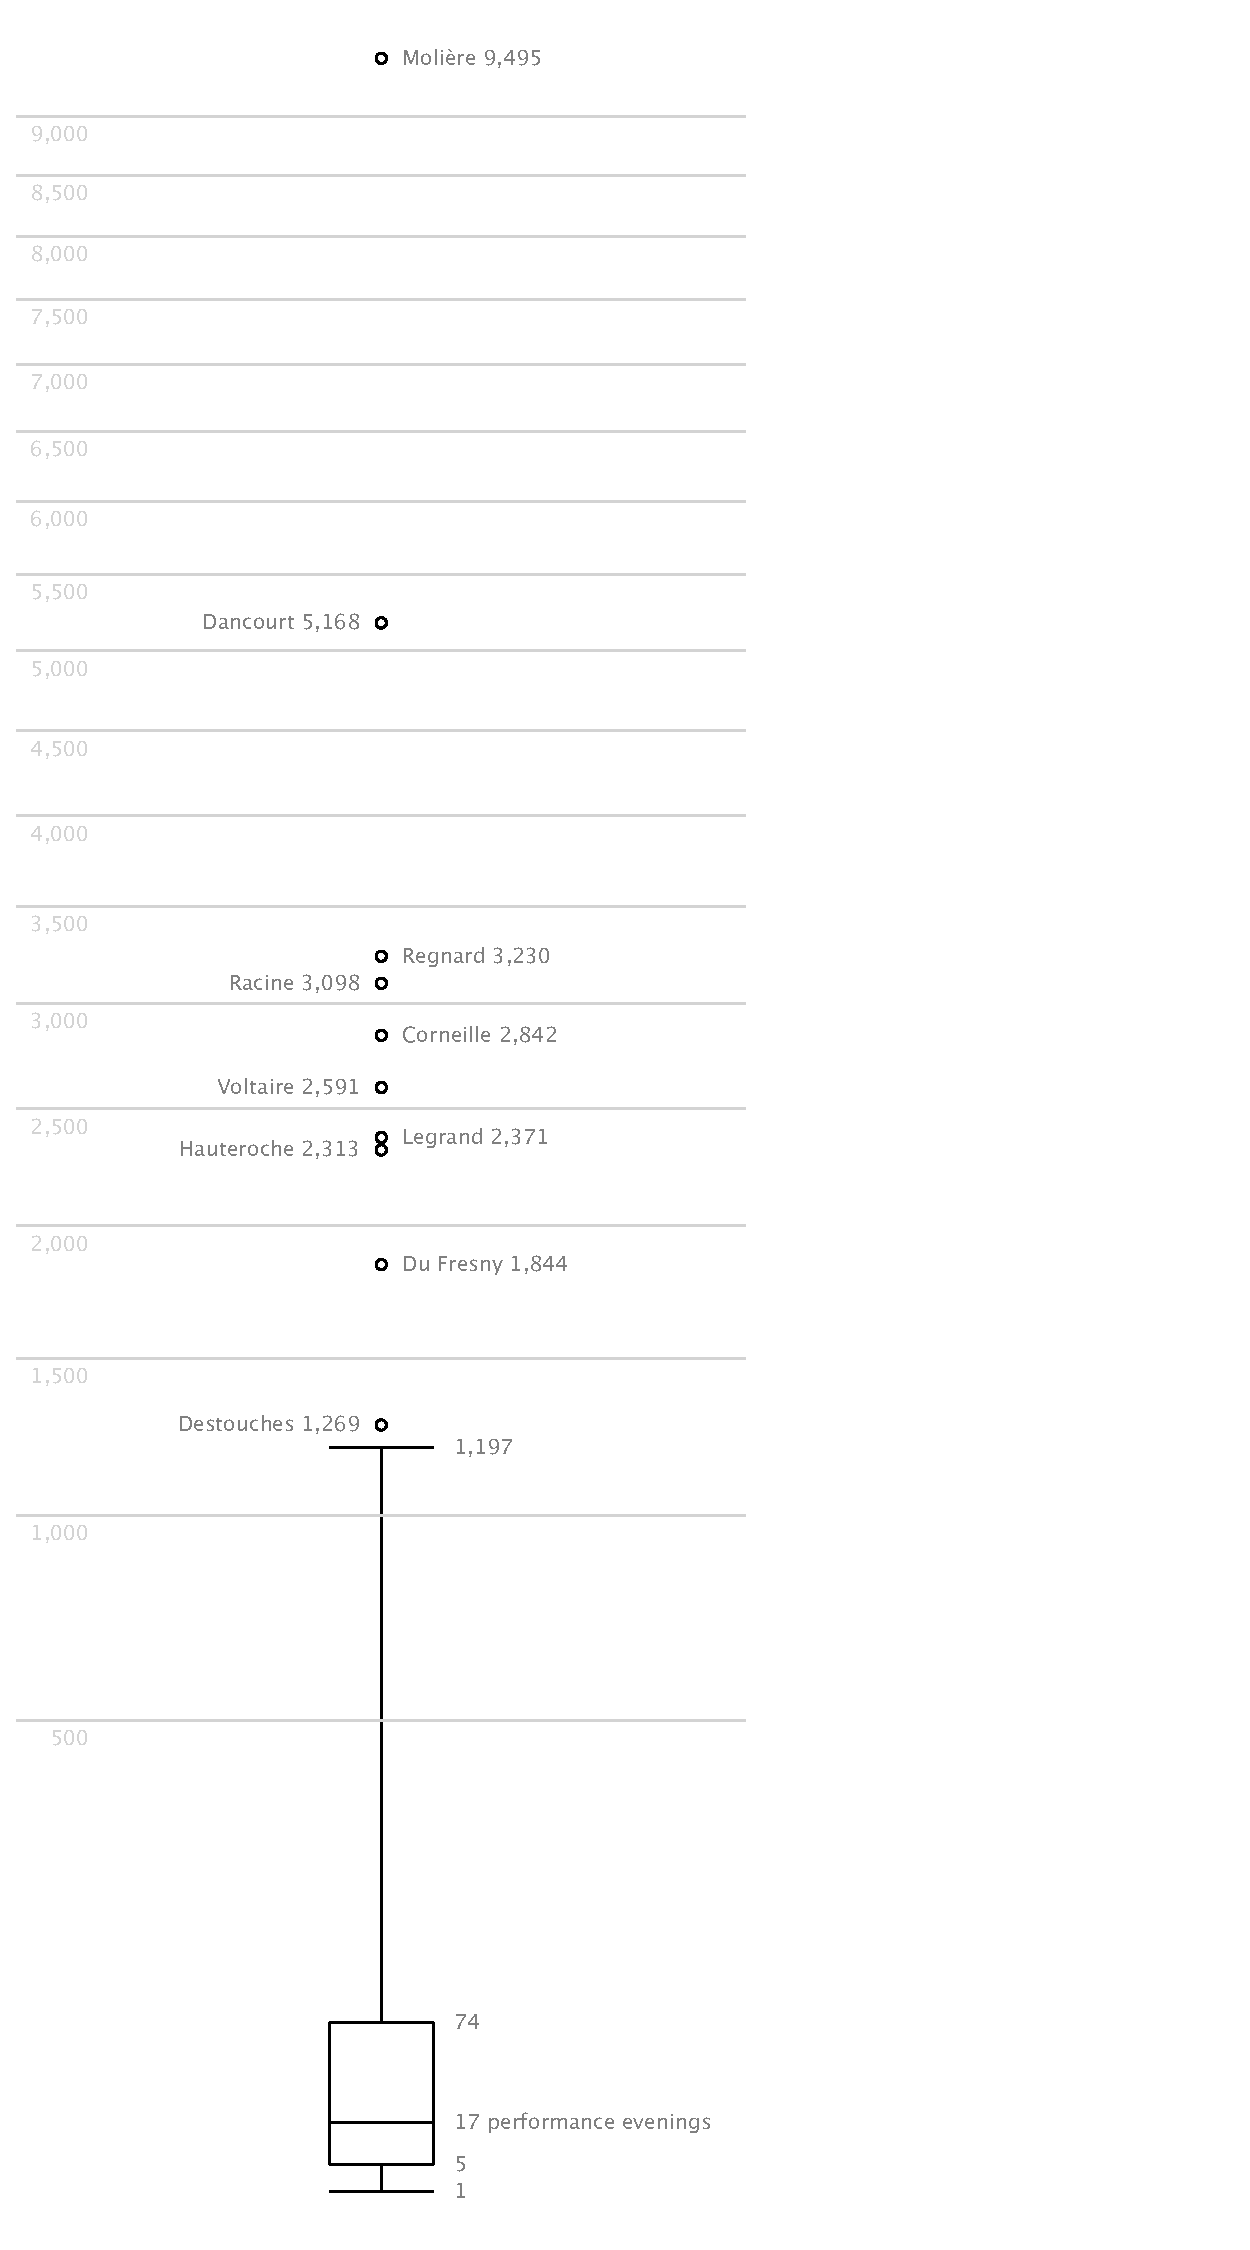
\includegraphics[height=9in]{viz/author_performances.pdf}
	\caption{Comédie Française authors by number of evenings performed}
  \label{fig:tukey_boxplot}
\end{figure}

Giving a sense of the overall landscape, while also providing opportunities to drill down and inspect specific features is a task in exploratory data analysis. This term, introduced by John Tukey in his 1977 book of the same title, encompasses a collection of techniques for identifying the main characteristics of a novel dataset, about which one may initially know nothing.  Tukey contrasted this exploratory process of surveying the data landscape and forming some initial hypotheses to confirmatory data analysis, the subsequent task of using data to confirm or disprove a hypothesis one has already formulated.\cite{TUKEY:1977}  The CFRP analytics site (http://christopheryork.github.io/cfrp-analytics/; http://cfregisters.org/app), which our theater student might use to generate many of the examples in this paper, was conceived as a general-purpose tool to enable users without a background in statistics to do basic exploratory data analysis—to formulate hypotheses, do confirmatory data analysis to test them, and then primary source critique to confirm that hypotheses are well-supported by the Comédie-Française’s archival resources.  It is this balance between data analysis and source critique that makes the CFRP analytics tool unusual, bridging statistics and the humanities.

Before we delve into description of the CFRP analytics tool, let’s pause first to consider potential visual displays for exploratory data analysis, so as to have a sense of the design space. Suppose our student has decided her best way into the Comédie-Française Registers data is to look at authors.  What sort of visualization can answer these questions: Which were the most prominent and influential authors?  How did minor authors fare in the repertoire?  What were the major periods, and how often did playwrights remain popular across periods?

When Tukey proposed exploratory data analysis as a field, he envisioned using visuals based on descriptive statistics as the primary entry point to new datasets.  For example, our student could start with the Tukey boxplot in figure \ref{fig:tukey_boxplot}, which uses the number of evenings the Comédie Française performed a play by the given author as a rough proxy for authorial importance.  Despite its visual spareness, the graph is information-rich, sketching the outlines of an theater troupe that experimented restlessly with new authors’ work but viciously dispatched unsuccessful ones after a few nights of poor performance; all the while staging works by the most successful authors over and over again. Of the 314 non-anonymous authors or co-author teams whose work played at the Comédie-Française between 1680-1793, fully 25\% had work in-theater for only 1 to 5 evenings (lower box edge).  Half of all authors saw 17 or fewer performances (median, the box’s center line), and 75\% of authors’ work had less than a full season’s time on the stage.  Clearly, success at the Comédie-Française was a vanishingly rare phenomenon.

At the upper end of the scale, Tukey’s visualisation singles out some outlier authors whose work was spectacularly successful.  Our student, while perhaps prepared for Molière’s pre-eminence, might be struck by the degree to which he dominated the Comédie-Française’s daily repertoire (note the exponential scale: Molière was performed fully twice as many nights as next-in-line comedian of manners Florent Carton Dancourt).

The striking success of Tukey’s visualisation lies in its balance between conveying the lay of the land—a large body of unsuccessful authors—while also singling out notable landmarks: individual authors whose work did succeed, and famously.  From this bit of exploratory data analysis, our imaginary student could begin formulating an overarching narrative while also following up on novel outlier authors whose names are unknown but whose success was clear: Destouches, Du Fresny, Hauteroche, Legrand, and so on.

Against the boxplot’s virtues, one can balance a number of demerits.  It is visually unsatisfying, rich in statistical implications but poor in visual detail that encourages users to look up new facts in a known resource.  Its very flexibility—we could be researching the distribution of genres, the profitability of individual plays, or variations in ticket price—begs for a visualisation tailored to the Comédie-Française alone.

Let us follow our hypothetical student to explore the top-performed Comédie-Française authors using a purpose-built visualisation for analysing repertoire (see figure
\ref{fig:heatmap}).  For each play by the 10 authors whose work was performed by the Comédie-Française more than 1,200 nights, this graph marks the number of performances per year onward from the premiere in a vertical line.  Stark differences in authorial profile and professional trajectory appear, which the previous graph had glossed over.  It becomes clear how dependent the Comédie-Française was on a canon of work already established before the formation of the troupe.  Of the authors whose plays were revived consistently, year on year through the troupe’s history, the lion’s share appear in the pivotal 1680-81 season: a large body of work by Molière, Pierre Corneille and Racine (at top).  Only Jean-François Regnard, gambler, adventurer and former slave turned playwright, was able to consistently introduce new hit plays that were revived year-on-year.  Voltaire, it becomes clear by comparison, only hit his stride in mid-career with Zaïre in 1732; his later plays languished, premiered but un-revived.

\begin{figure*}
  \centering
	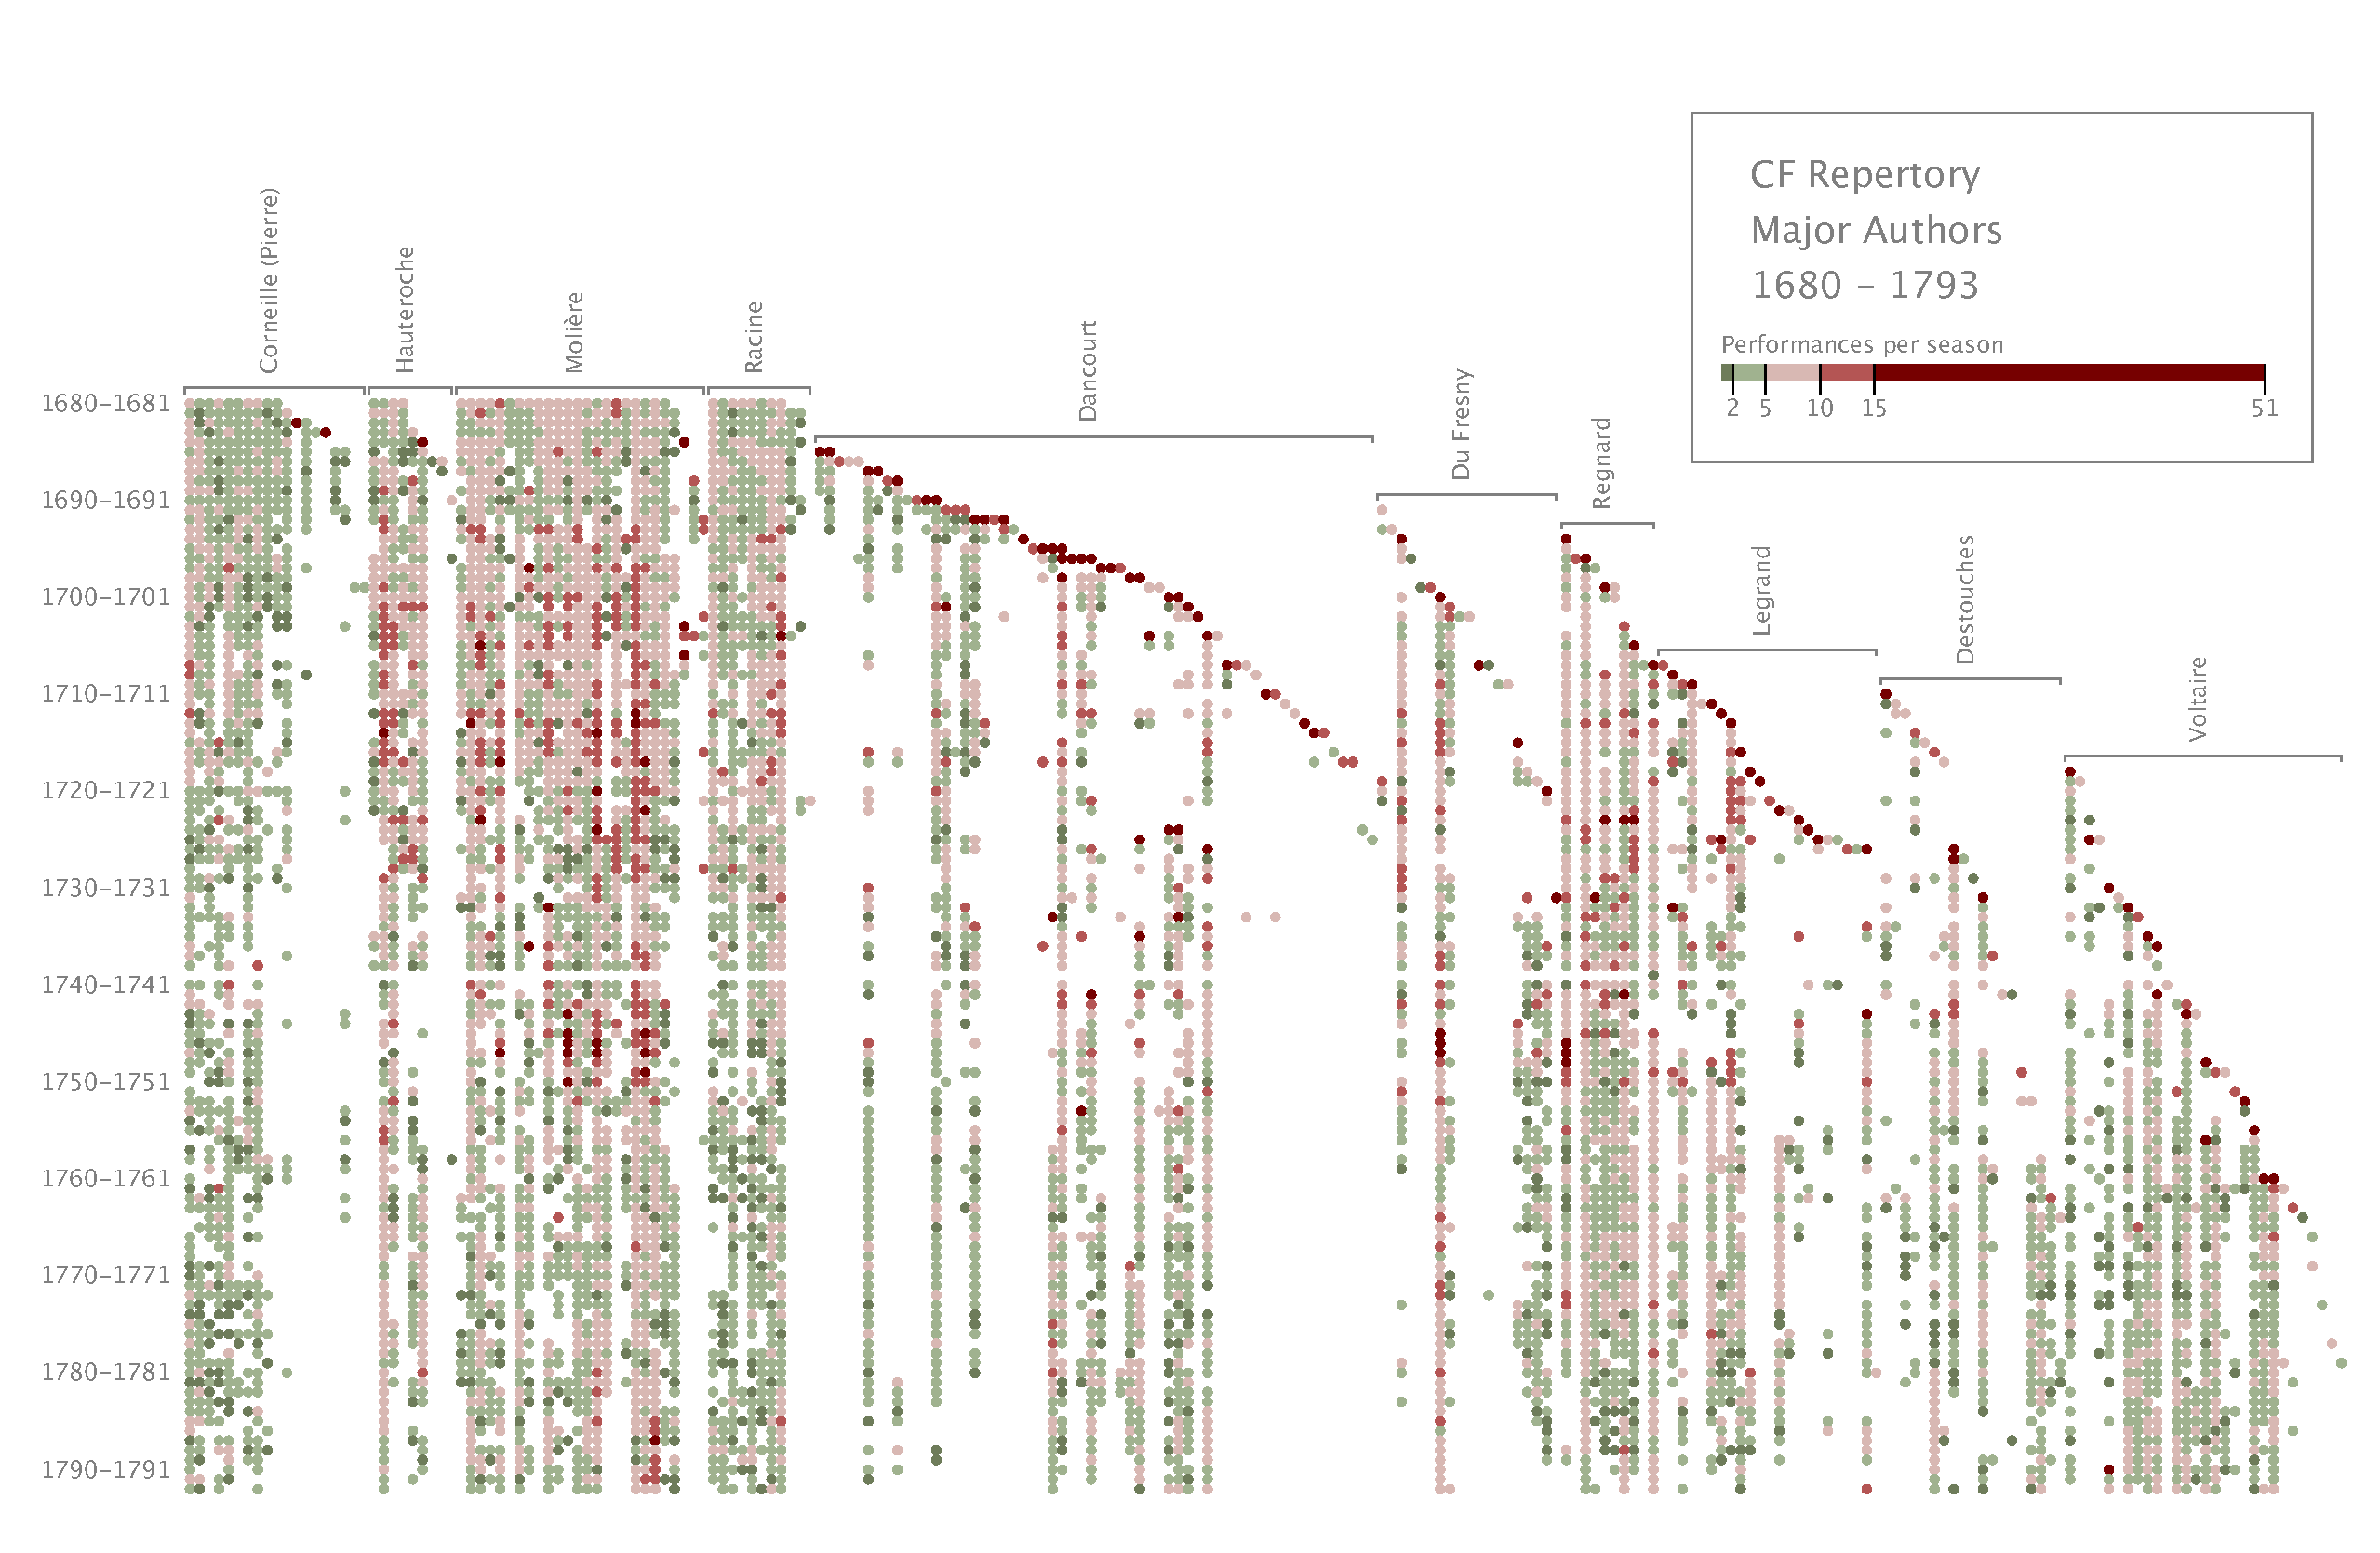
\includegraphics[width=10in,angle=270]{viz/repertoire_by_season.pdf}
	\caption{}
  \label{fig:heatmap}
\end{figure*}

From a purpose-built visualisation such as this, our hypothetical student might make any number of observations that open doors into individual authors’ professional careers.  Pierre Corneille’s frustrated later-life failures are clearly visible; as is Dancourt’s unique authorial signature as a fount of works consistently premiered year on year, yet only intermittently canonised.  Likewise, Abraham-Alexis Quinault’s (also known as Dufresne) status as the one-hit wonder author of Esprit de Contradiction is confirmed.  More subtly, one sees the gradual shift in taste away from classical models, from Molière’s singular dominance of repertory through 1720, to a more tepid (but consistent) series of revivals after 1750—just as Voltaire’s work achieved dominance.

The heatmap’s visual richness and usefulness for investigating authorial history hide faults that make it quite unsuitable for exploratory data analysis.  As noted above, a cardinal virtue of the author performance boxplot was balance between giving a sense of the ``landscape'' of all authors’ performance histories while simultaneously singling out notable features: ten particularly well-performed authors.  The heatmap’s balance of dark and light suggests similar reading—but deceptively.  Because it does not include all plays performed through the 113-year sequence of the Comédie-Française dataset, it gives little sense of why these are of particular interest: where, how many, and what characterised the unsuccessful authors?

It is a picture of some tall trees in isolation from the surrounding forest.  One might think that including every play and ordering them in sequence chronologically by premiere would counteract this (see figure \ref{fig:heatmap_all}).  While it does accurately suggest the balance between often-performed plays dating from the years of the troupe’s founding and rarely-revived plays that premiered later, to see this effect we must order by the year each play’s premiere and so lose the grouping by author.  Some of the most important features of the dataset disappear: for example, Voltaire’s dominance of the post-1730 repertoire is completely hidden, since his successful plays are scattered among many less-successful ones by other authors.

\begin{figure}
  \centering
	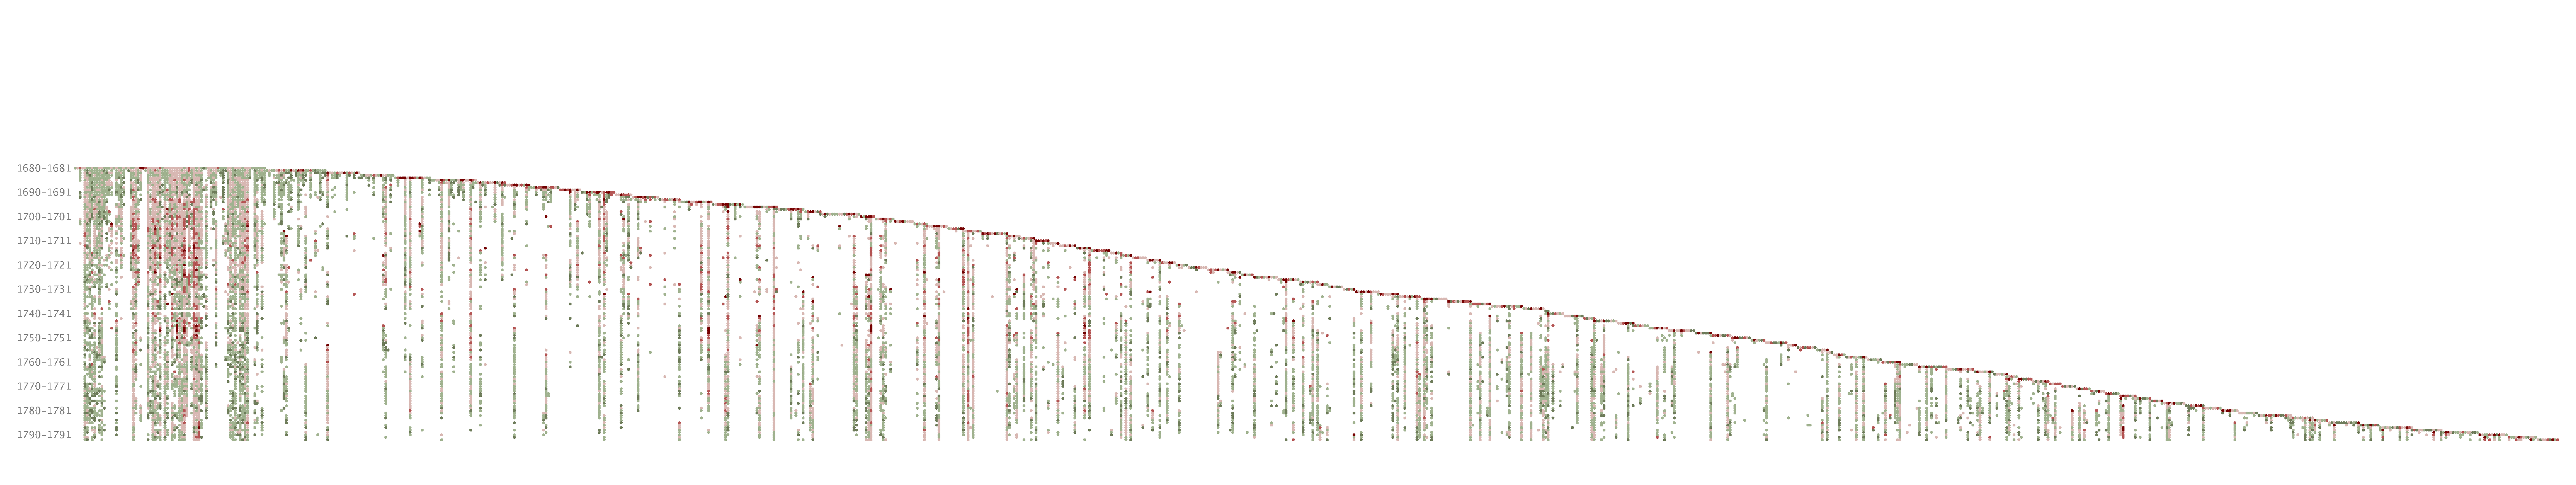
\includegraphics[width=9in,angle=270]{viz/repertoire_by_season_all.pdf}
	\caption{\color{red}Complete CF repertory arranged by year
	         \newline
					 \color{black}(Ineffective views of data provided for comparison will be captioned in red.)}
  \label{fig:heatmap_all}
\end{figure}

Perhaps more damning, the repertoire heatmap in figure \ref{fig:heatmap} is a special purpose visualisation, crafted to expose a fixed set of patterns but difficult to adapt to other categories of analysis.  Changing it to look at the genre of plays performed over time, or variations of what is played during a week, would basically require starting over with a novel programming task.  By contrast, during the process of exploratory data analysis, users are likely to want to experiment with many different aggregations and graphs in a short period of time—for example, to see ``were plays of a different genre performed in later decades?'' or ``were different weekdays associated with different genres?''  Despite involving the same variables—time and genre of play performed—these two questions lend themselves to different analyses and graphs.  This is because ``decade of performance'' is a linear and continuous aspect of the data, while ``weekday of performance'' is cyclical and discrete.

\subsection*{Goal and Design Constraints: General vs Special-Purpose Tools}

A digital humanist with specialist skills in statistics and data visualisation, given the Comédie-Française dataset and a research question like the ones above, might produce any number of compelling purpose-built visuals that speak compellingly to questions like ``how did genre vary by weekday'' or ``which were prominent authors performed by the troupe?''  The challenge for an exploratory data analysis tool, however, is to enable the non-specialist user to probe any number of different questions using general-purpose visuals.  (For one potential starting list of questions for the Comédie-Française dataset, see the sidebar).

Doing so involves comparing any number of different aspects of the dataset in quick succession, digging for suggestive features and large-scale patterns, formulating, testing and rejecting many hypotheses.

The tool works by progressive refinement of the dataset, to expose distributions of the data points across a number of dimensions (listed in the sidebar).  Let us follow the prior query through, to show how our student user might use the tool to explore the problem of determining the main authors in the Comédie-Française’s repertoire, their periods and relative importance.

To begin, our student would select an aggregate value of interest: for example, the number of performances; gross receipts; average price of tickets sold; or average receipts per night.  As seen in the Tukey boxplot we considered first, number of performances is a good initial metric indicating the prominence of an author in the repertoire.  On choosing this, our student sees the entire dataset aggregated by number of nights performed: over the 114-year period covered by the dataset, the Comédie-Française performed 34,904 nights (figure \ref{fig:opening}).  At about 306 live evenings per year (34,904 / 114), this already gives some indication of the theater’s preternatural activity.  Was the Comédie Française pressed to maintain profitability by keeping its doors open and attendance consistently high, a stress familiar to 20th century theater owners?  Our student investigator does not know; but already a field of questions is opening up that supplements her initial interest in repertoire.  What role did prominent authors play in maintaining the Comédie Française’s yearly schedule?

\begin{figure}
  \centering
	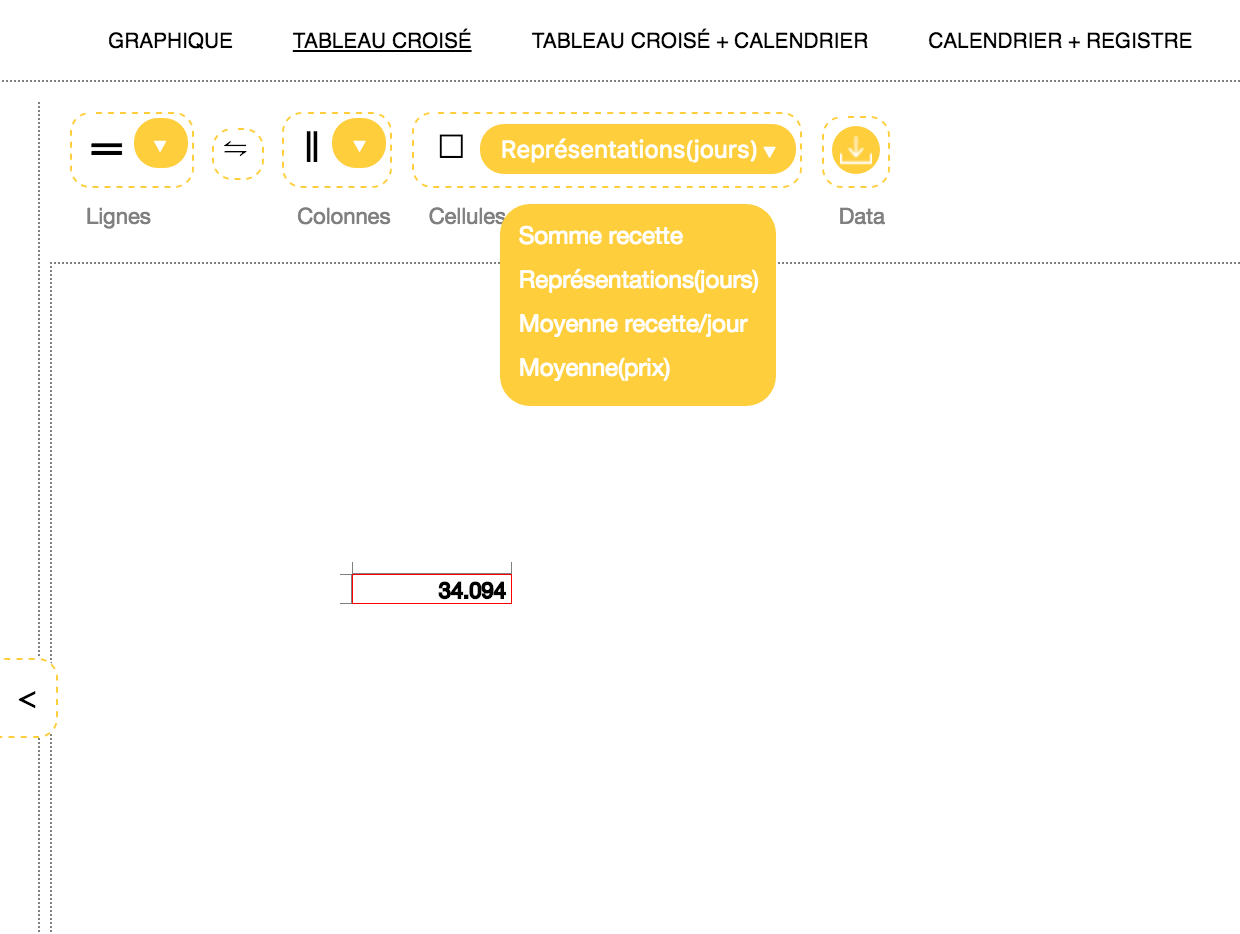
\includegraphics[width=3.25in]{steps/opening.png}
	\caption{}
	\label{fig:opening}
\end{figure}

Our student decides to take a quick look at how the number of performances varied over the course of the theater’s history.  From the list of available dimensions, she elects to divide the existing result by decades (figure \ref{fig:dimensions}).  This will give a sense of how performances were distributed through history (figure \ref{fig:performances_by_decade}).  While this is an obvious—and good—choice, our student could have chosen to drill down into the dataset using any of the other dimensions available: to see which genres were performed more nights, for example, or to find the most (or least) popular play titles by number of performances.

\begin{figure}
  \centering
	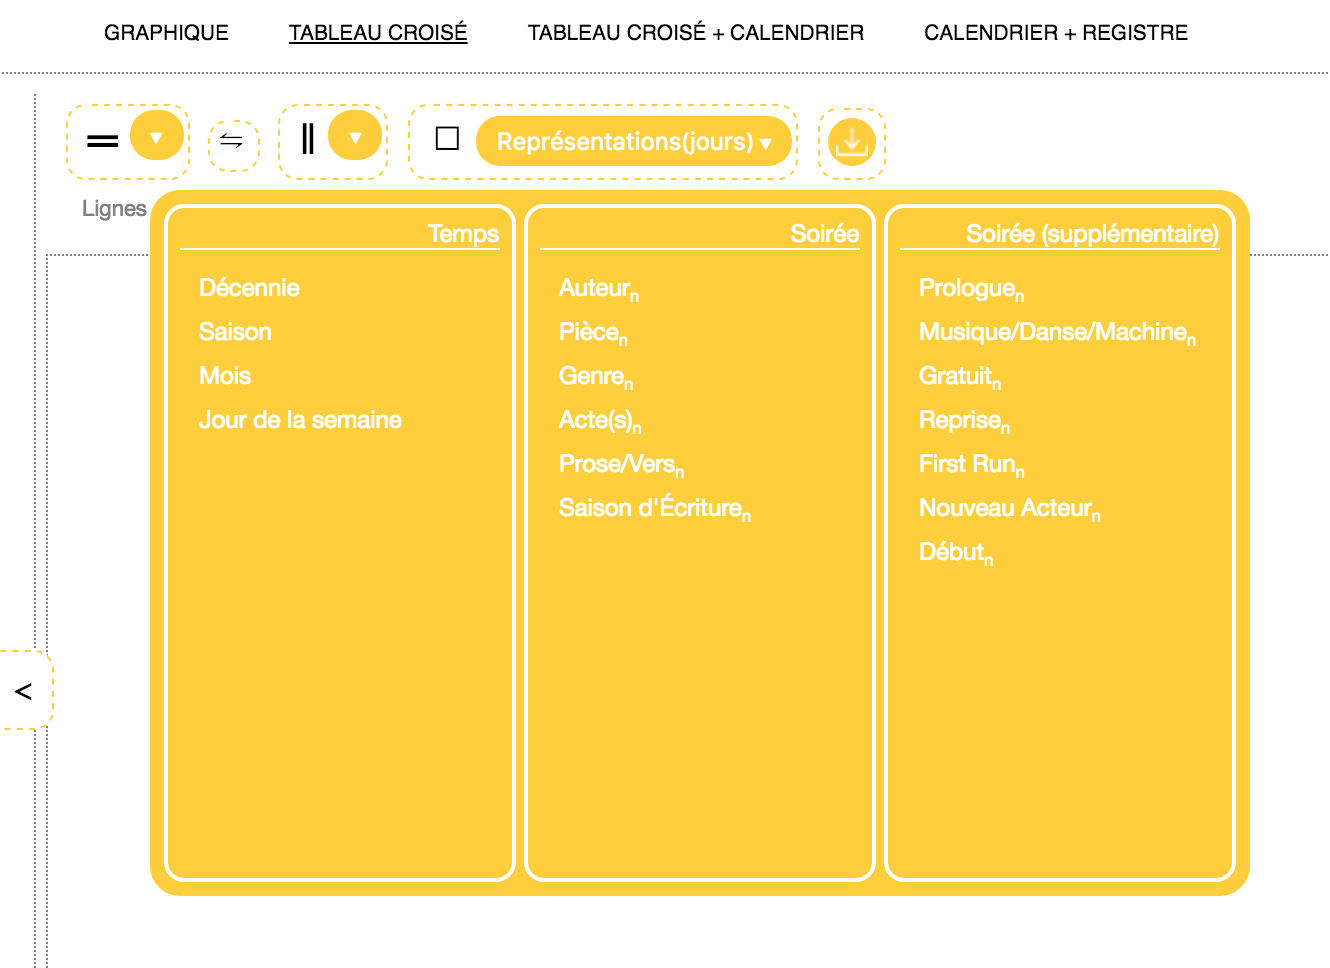
\includegraphics[width=3.25in]{steps/dimensions.png}
	\caption{}
	\label{fig:dimensions}
\end{figure}

\begin{figure}
  \centering
	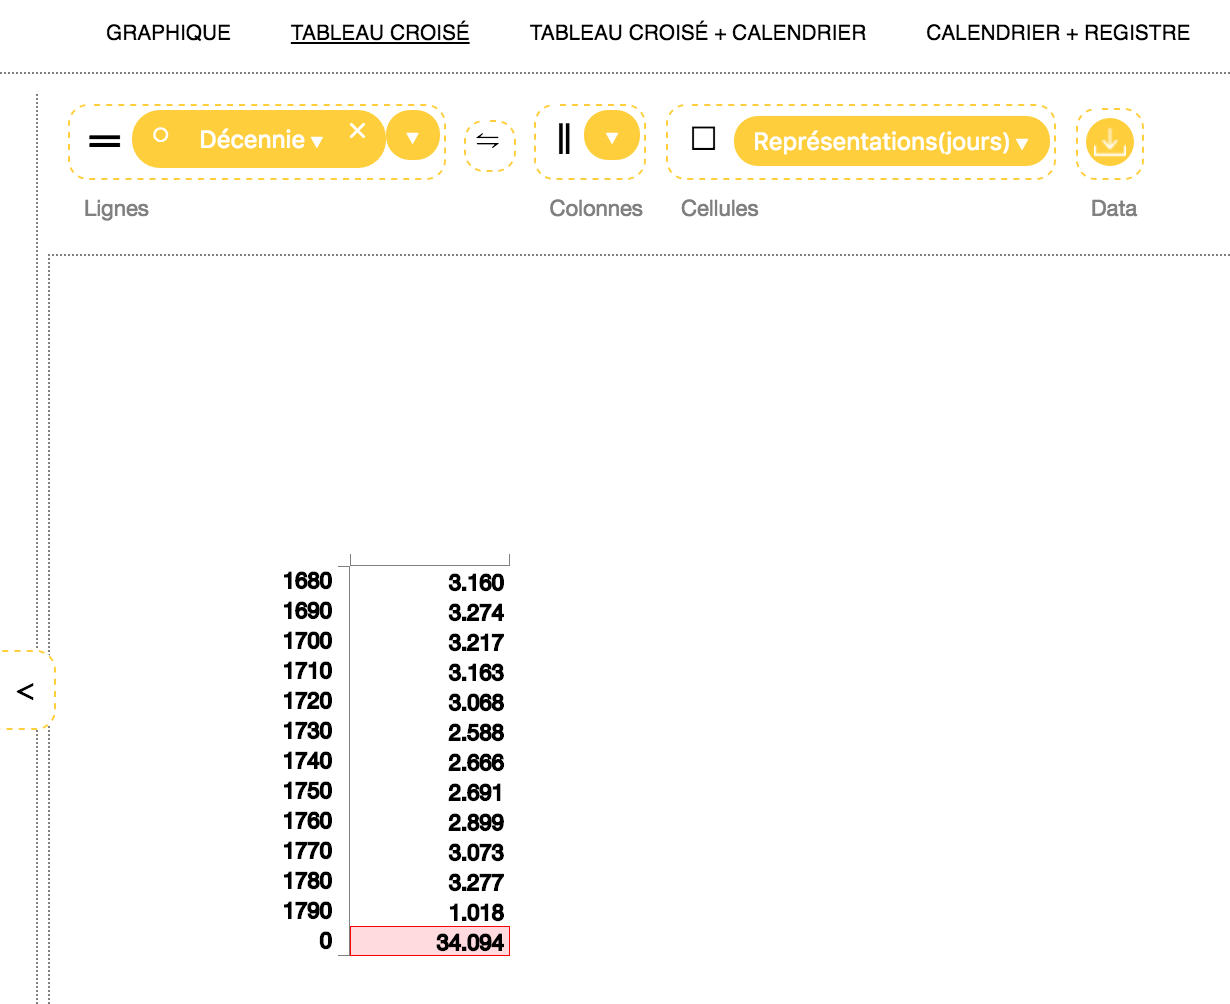
\includegraphics[width=3.25in]{steps/performances_by_decade.png}
	\caption{}
	\label{fig:performances_by_decade}
\end{figure}

Seeing results in tabular form can be useful, particularly when one delves deep into a particular problem or research question.  A visual presentation gives more immediate meaning to the same set of numbers, however.  From here, we will follow the student as she does exploratory data visualisation using the tool’s graph component, which she accesses by choosing the leftmost results panel (figure \ref{fig:performances_by_decade_graph}).
\todo[noline]{correct line graphs: 1790 datapoint is misleading because this decade includes fewer years.}

\begin{figure}
  \centering
	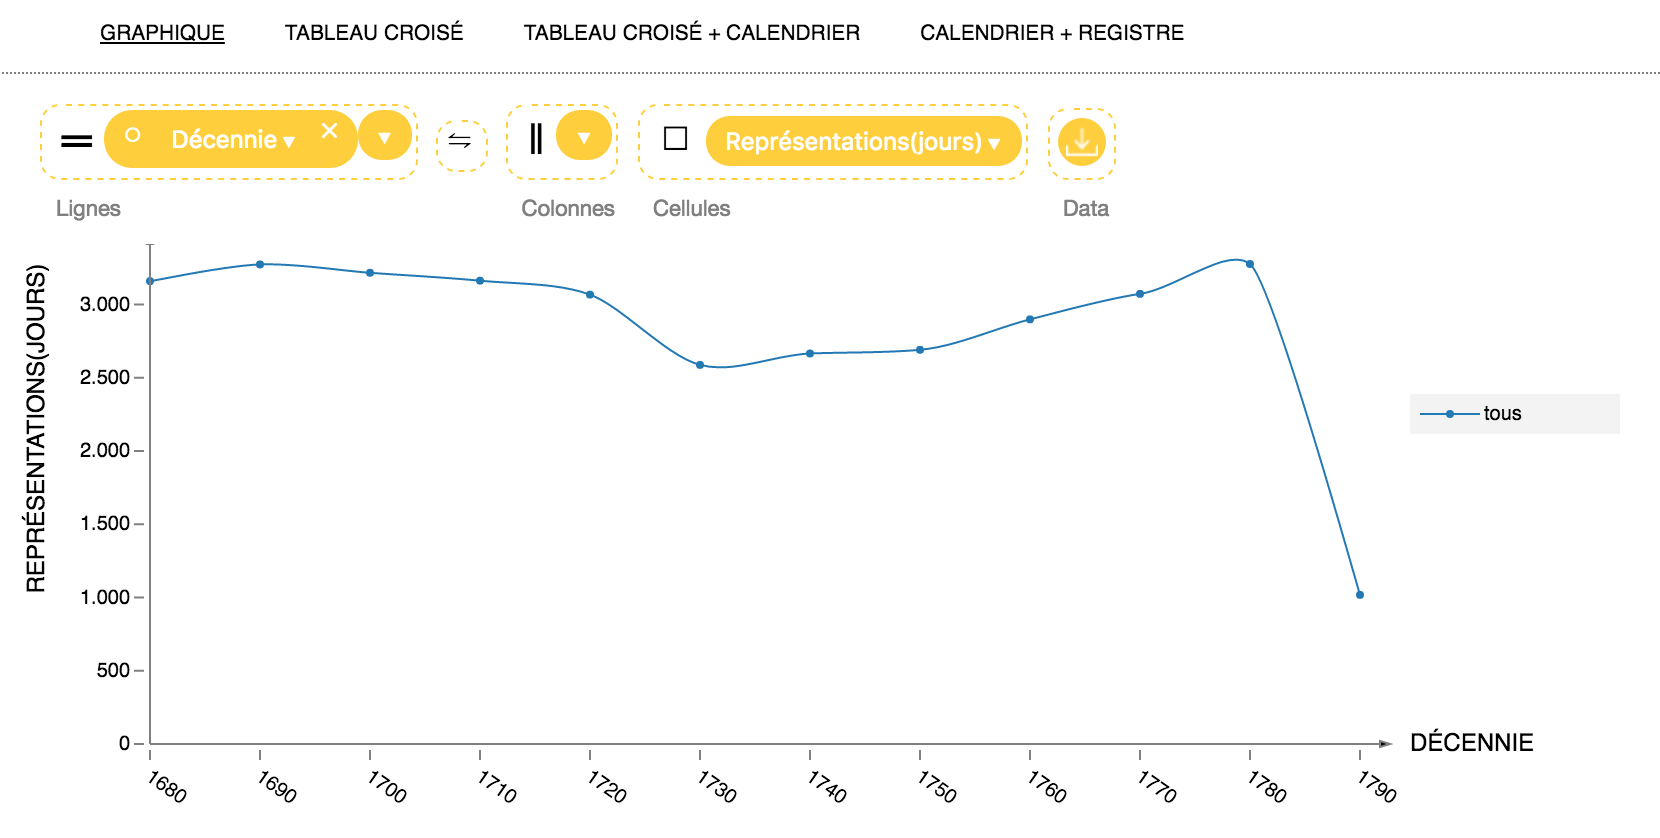
\includegraphics[width=3.25in]{steps/performances_by_decade_graph.png}
	\caption{}
	\label{fig:performances_by_decade_graph}
\end{figure}

The graph of number of performances by decade is immediately more suggestive than the table of numbers.  The much lower number of performances in the 1790s immediately stands out, but even more striking is the slight fall in activity at 1720, which only gradually rises back to its original levels at the turn of the 19th century.  However, our student is immediately struck by the years immediately preceding the French Revolution, when it is clear the theater thrived.  Is it possible, the Comédie Française was involved in and benefited materially from the intellectual and political turmoil of the Enlightenment?

Perhaps this question will become clearer as our student pursues her original interest in the Comédie Française’s prominent authors.  She chooses to divide the current query on performance evenings per decade further, this time by the authors of the plays performed.

\begin{framefloat}[b]
	\fontsize{8pt}{8pt}\selectfont
  \begin{description}[noitemsep,align=left]

		\item[Measures]
			\item number of performances (evenings)
			\item gross ticket receipts
			\item mean ticket receipts per night
			\item mean price per ticket sold
			\item weighted ticket receipts

    \vspace{10pt}
		\item[Dimensions]
			\item play
			\item author
			\item title
			\item acts
			\item genre
			\item style: prose or verse
			\item performance
			\item debut, reprise, firstrun, new actor/role
			\item seating category

    \hrulefill
		\item[Facts]
			\item date
			\item number of tickets sold
			\item price per ticket
  \end{description}
\end{framefloat}

She chooses the default option for ``author'' (author\textsubscript{n}, explained further below) in the table’s columns.  This generates a table of number of performances for each author, divided by decade.  Because there are 314 columns in this table, it is excerpted in figure \ref{fig:stitched-author-table}.

\begin{figure*}
  \centering
	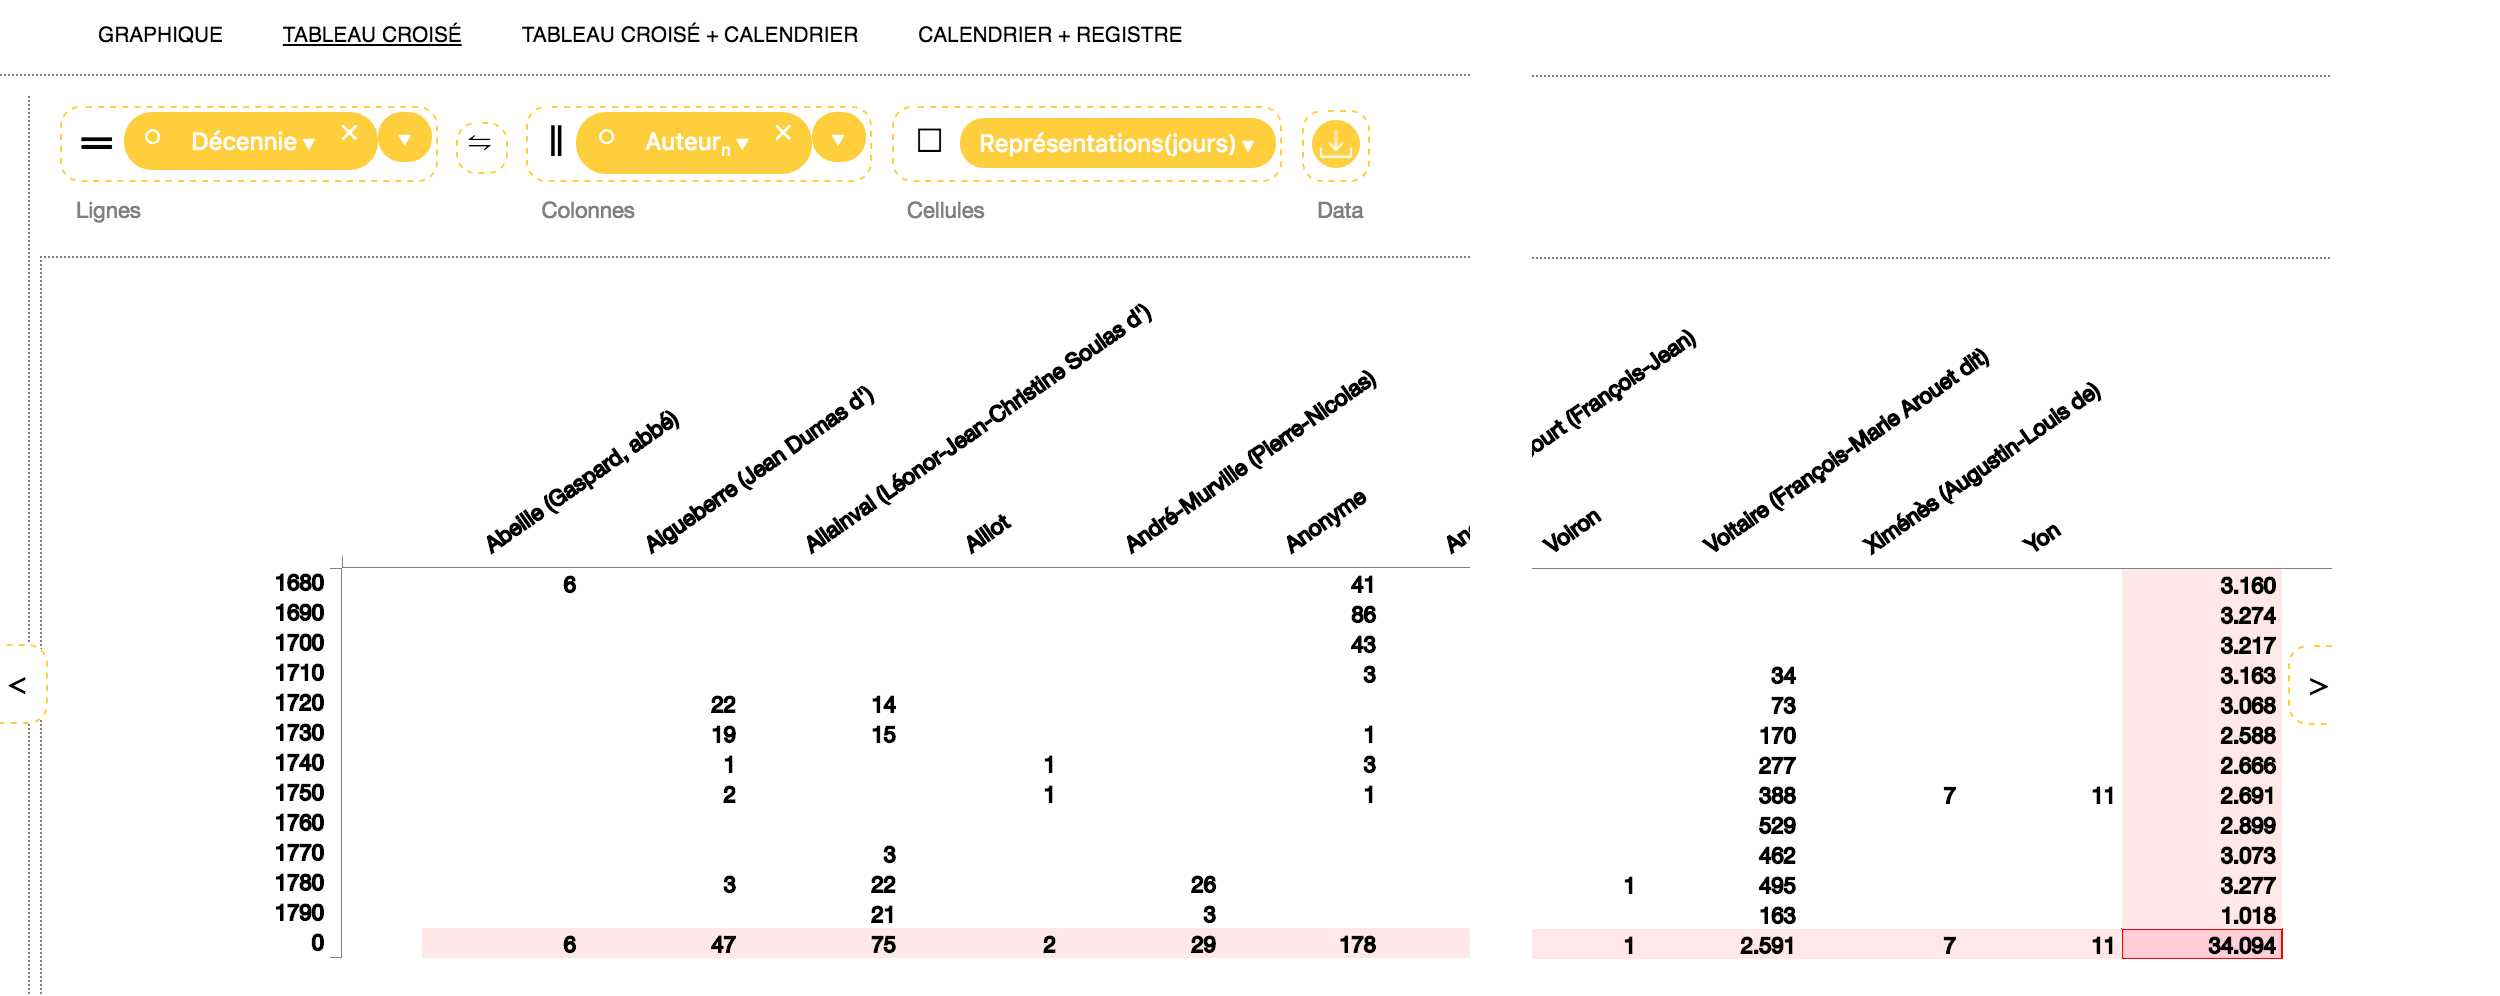
\includegraphics[width=7in]{steps/stitched-author-table.png}
	\caption{}
	\label{fig:stitched-author-table}
\end{figure*}

Subtotals tallied by author appear at the lower margin of the table, and tallied by decade at the right margin; the lower right cell tallies performances for the entire table.  Authors are ordered alphabetically across the top, such that as the user scrolls horizontally, it is possible to detect from visual density of the figures which were the prominent authors, and in which decades.  In this table, for example, Voltaire’s dominance of the repertoire from the 1730s onward is immediately obvious.

Visual inspection only conveys a rough sense of the historical distribution of performances between authors, however.  It would be more helpful to know immediately which were the most- and least-performed authors.  To accomplish this, the student sorts the table by column (author name), as seen in figure \ref{fig:sorted}.  Here, we begin to see the outlines of the vital descriptive statistics that John Tukey foregrounded in his boxplot.  As can be seen by comparison with figure \ref{fig:tukey_boxplot}, the sorted crosstab table identifies notable outlier datapoints along a dimension.  From here, our student can begin making interpretive inferences like those we pointed out in our discussion of Tukey’s boxplot: Molière’s central place in the repertoire is immediately obvious, as is the prominence of the other foundational authors like Racine and Corneille right from 1680.  Moreover, some of the phenomena we observed in the custom-tailored heatmap (figure \ref{fig:heatmap}) are evident here, but hidden in the boxplot: for example, Voltaire’s gradual rise to fame at 1750, when his importance in the repertoire superceded that of Racine and Corneille together.  (By sorting the table in the opposite order, low-to-high by columns, our student can also explore the least-performed authors, exposing  the fragmentation and churn we noted in the Comédie Française repertoire using Tukey’s boxplot.)

\begin{figure}
  \centering
	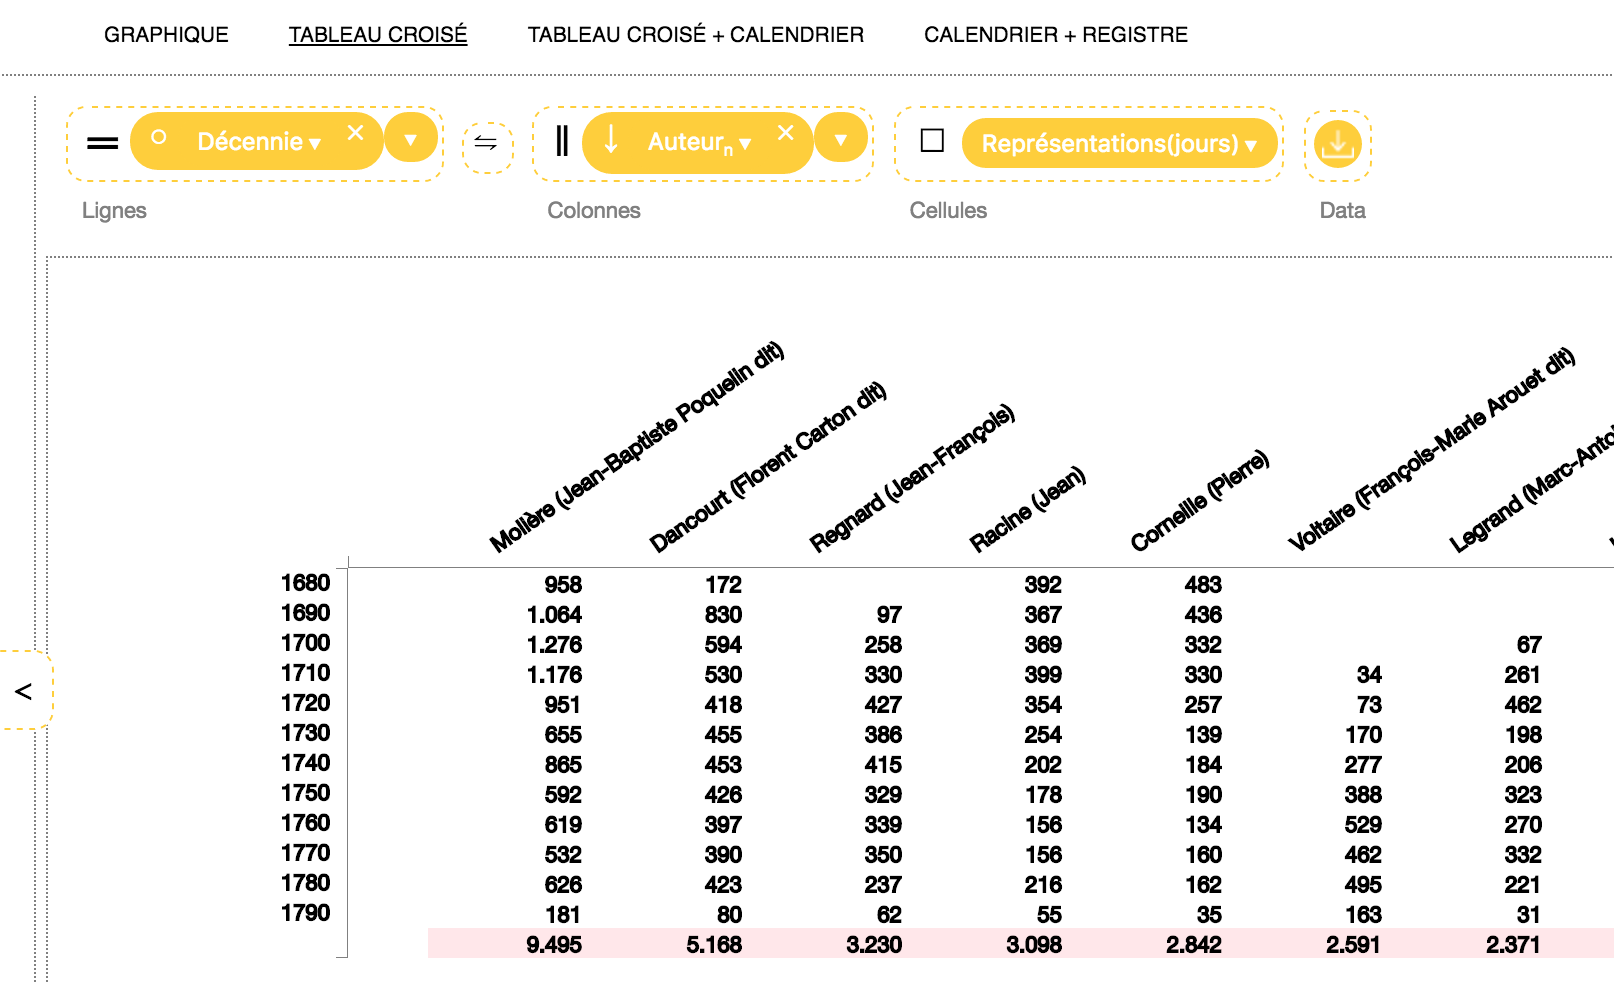
\includegraphics[width=3.25in]{steps/sorted.png}
	\caption{}
	\label{fig:sorted}
\end{figure}

One of the cardinal advantages of the Tukey boxplot, as we noted, lay in giving a sense both of absolute numbers of performances for each author, as well as how those numbers compared with the body of other authors in the repertoire.  While the table format, with fixed ordinal positions for rows and columns, cannot mimic this graphically, it can convey a sense of the importance of each value within the population of an entire row or column.  Doing this enables our student to compare the relative prominence of high-performed authors to each other, and to the entire population of authors per decade (step \ref{fig:percents}).  Here she sees her intuitions about the troupe’s dependence on Molière confirmed: fully 28\% of all nights through the run saw the performance of a Molière play (lower-right corner), as against 7.6\% of all nights for Voltaire.  More importantly, she now has a sense of the significance of Voltaire’s rise after 1750: in this and succeeding decades, between 14-16\% percent of all nights involved a performance of one of his plays.  However, decade by decade through Voltaire’s heyday, it becomes clear that Molière plays still formed a higher proportion of the repertoire.  Looking at the top-performed authors as a group makes this conservative phenomenon even further.  The top 6 authors appeared on fully 60-80\% of all nights!
\todo{double check this works with author\_n}

\begin{figure*}
  \centering
	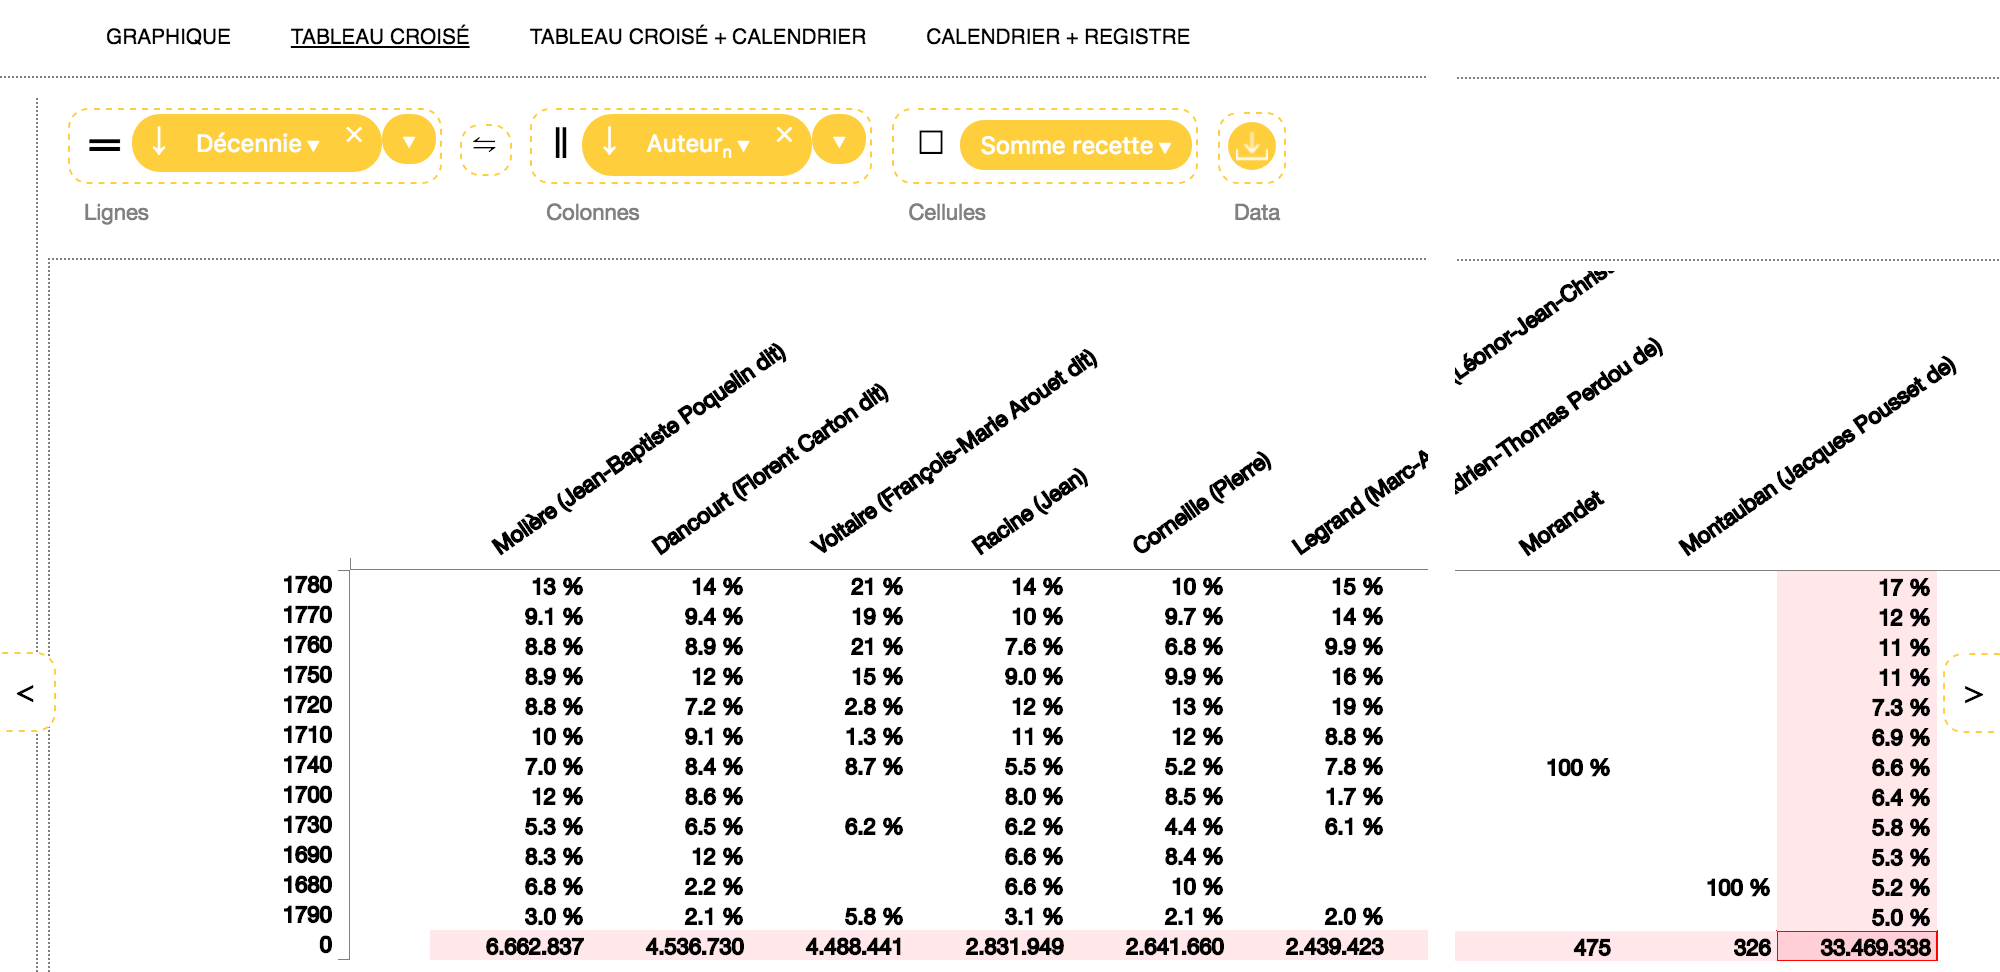
\includegraphics[width=7in]{steps/percents.png}
	\caption{Per-author distribution of play performances, for each decade}
	\label{fig:percents}
\end{figure*}

Looking back at our student’s progress using cross-tabulations, it is clear her insights are built on three vital features.  First, the ability to divide the dataset by more than one dimension (in this case, by author and time rather than just author).  Second, sorting from high-to-low and low-to-high values on an axis make it easy to locate the top and bottom performers (these are generally Tukey’s statistically-significant outliers).  This enabled our student to identify notable authors without having to scan the entire table. Third, showing computed aggregates ranked as proportion of a row or column of the data gives a sense of how important each value is vis-a-vis its neighbors.  Hence our student could judge the relative prominence not only of Voltaire to Molière, but also each of these authors compared with the unseen collection of all Comédie-Française authors.

Shortcomings of the table format quickly appear, however, if our student moves from comparing authors performances by decade to each other, to comparing authors’ performances rates in one decade to those in other decades.  When, for example, was the peak in Comédie-Française performances and did it correlate with a particular author?  To begin looking at this question, the student changes the table above to order and calculate percentages within columns rather than rows (figure \ref{fig:stitched-decades-table}).
\todo[noline]{table should show performance count, for comparison with figure \ref{fig:percents}.}

\begin{figure*}
  \centering
	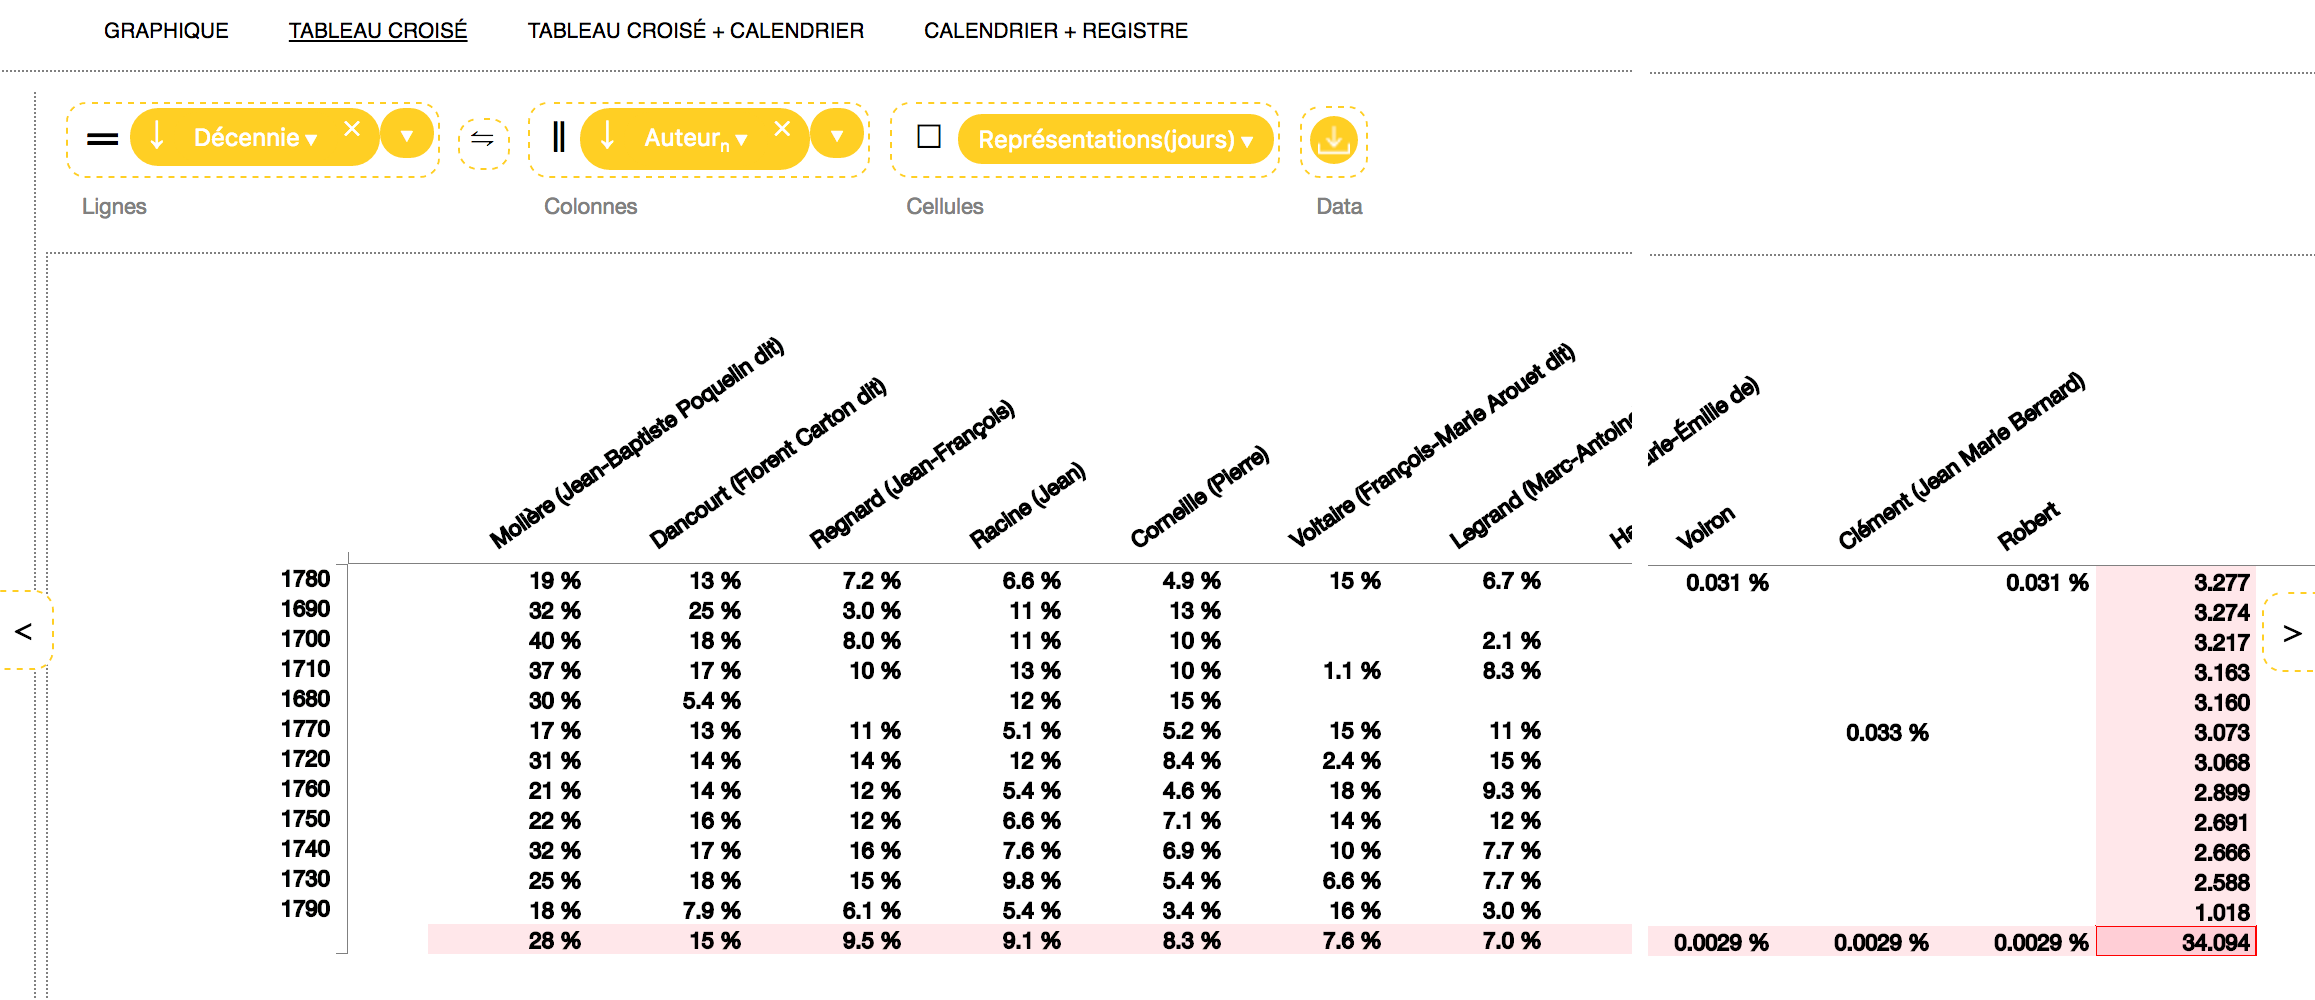
\includegraphics[width=7in]{steps/stitched-decades-table.png}
	\caption{\color{red}Per-decade distribution of plays performed, for each author}
	\label{fig:stitched-decades-table}
\end{figure*}

While the display conveys the information our student seeks—which decades saw the most open performances, broken down by author—it feels incoherent, because unlike ``author’s name'', ``time'' has a natural order and we expect to always see data presented in that order, even when seeking minima and maxima.  Ordering clearly matches the rising trend of more and more performances in each successive decade from 1740 to 1780 (see the far right column): however, we still expect to see decades plotted in chronological order so we can seek limits visually.

In this case, a simple line or scatter graph (e.g. figure \ref{fig:performances_by_decade_graph}) immediately immediately draws the eye to high and low values, even though the computer has not been instructed to highlight them by sorting or special marks.  Clearly when exploring data in a continuous, ordered domain plots are more effective than tables of numbers: our student already noted the ease with which highs and lows can be read from a graph showing the per-decade count of evening performances (figure \ref{fig:performances_by_decade_graph}), as compared with the identical table (figure \ref{fig:performances_by_decade}).

However, if our student divides this graph of total performances by author, in an attempt to explore the prominence of individual authors across each decade of the Comédie Française's history, she obtains a result whose visual density clearly makes for sub-optimal data analysis (figure \ref{fig:author-performances-all}).  Some suggestive characteristics that we explored using the Tukey box-plot (c.f. figure \ref{fig:tukey_boxplot}) are  present: clearly one author dominated the repertoire in every season (blue line at top), while others seemingly grew in popularity to become box-office standards (red), sometimes entering this trajectory well into the Comédie Française's history (green).  Against these statistically-significant and highly-successful outliers, we see the main body of authors below, most of them performed under 100 times a season.  Finally, one of the most striking aspects of the Comédie Française's repertoire - the prevalence of authors whose plays saw under 10 performances - is completely hidden, due to the sheer density of lines at the bottom of the graph.

For the purposes of exploratory data analysis, it is useful to highlight top- and bottom-scoring trends and leave the overall distribution for later investigation.  (For example, a useful tool for working with the Comédie Française dataset should immediately expose Molière's dominance of the daily repertoire, even while allowing students to drill down to less-succesful authors).  Figure \ref{fig:top-author-performances} illustrates this approach, as deployed by the CFRP analytics tool: from figure \ref{fig:author-performances-all}, it graphs only the lines with the top 10 highest points, which it then labels in order.  The result gives a clear picture of which were the most prominent authors, together with the personal career trajectory for each: the red, blue and green outliers noted above are of course Molière, Dancourt and Voltaire.  While not as graphically rich as a purpose-built visualisation such as figure \ref{fig:heatmap}, for the purposes of interactive data analysis such a graph handily balances legibility with flexibility and utility.  From here our student might drill down to explore the history of a specific author; or re-sort to look at the 10 least frequently performed authors; or switch to look at another variable such as genre or ticket receipts.

\begin{figure*}
  \centering
	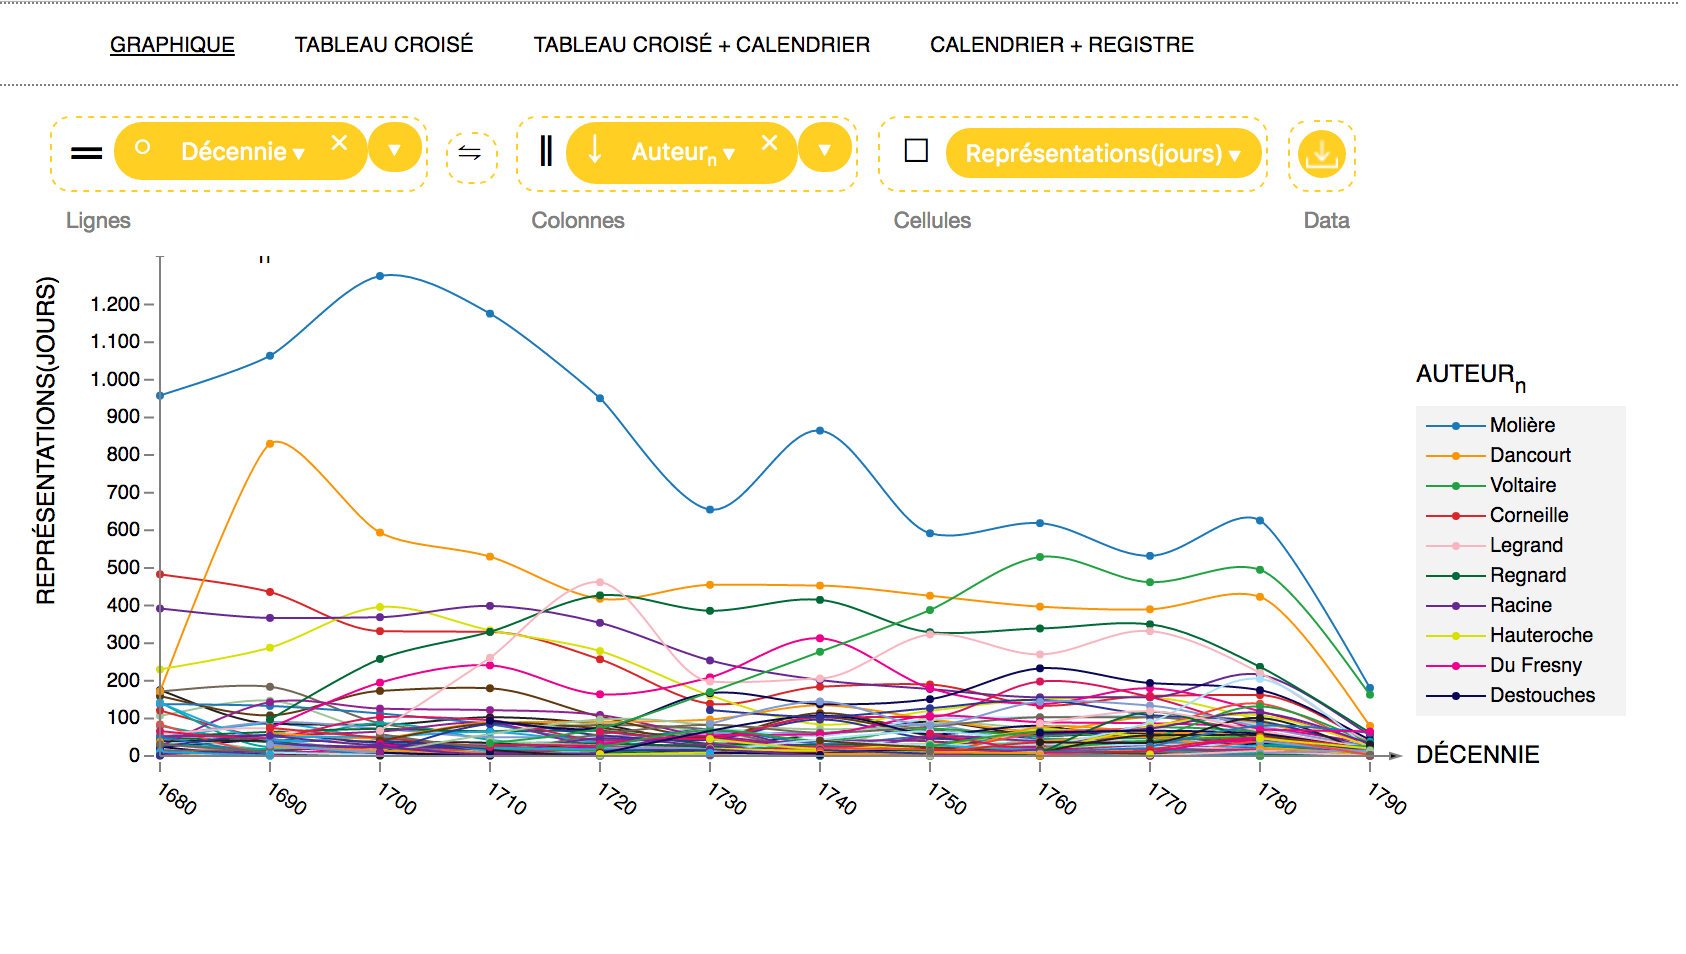
\includegraphics[width=7in]{steps/author-performances-all.png}
	\caption{\color{red}A plot that illustrates the utility of highlighting outlying high values, but obscures the overall distribution of the data.}
	\label{fig:author-performances-all}
\end{figure*}

\begin{figure*}
  \centering
	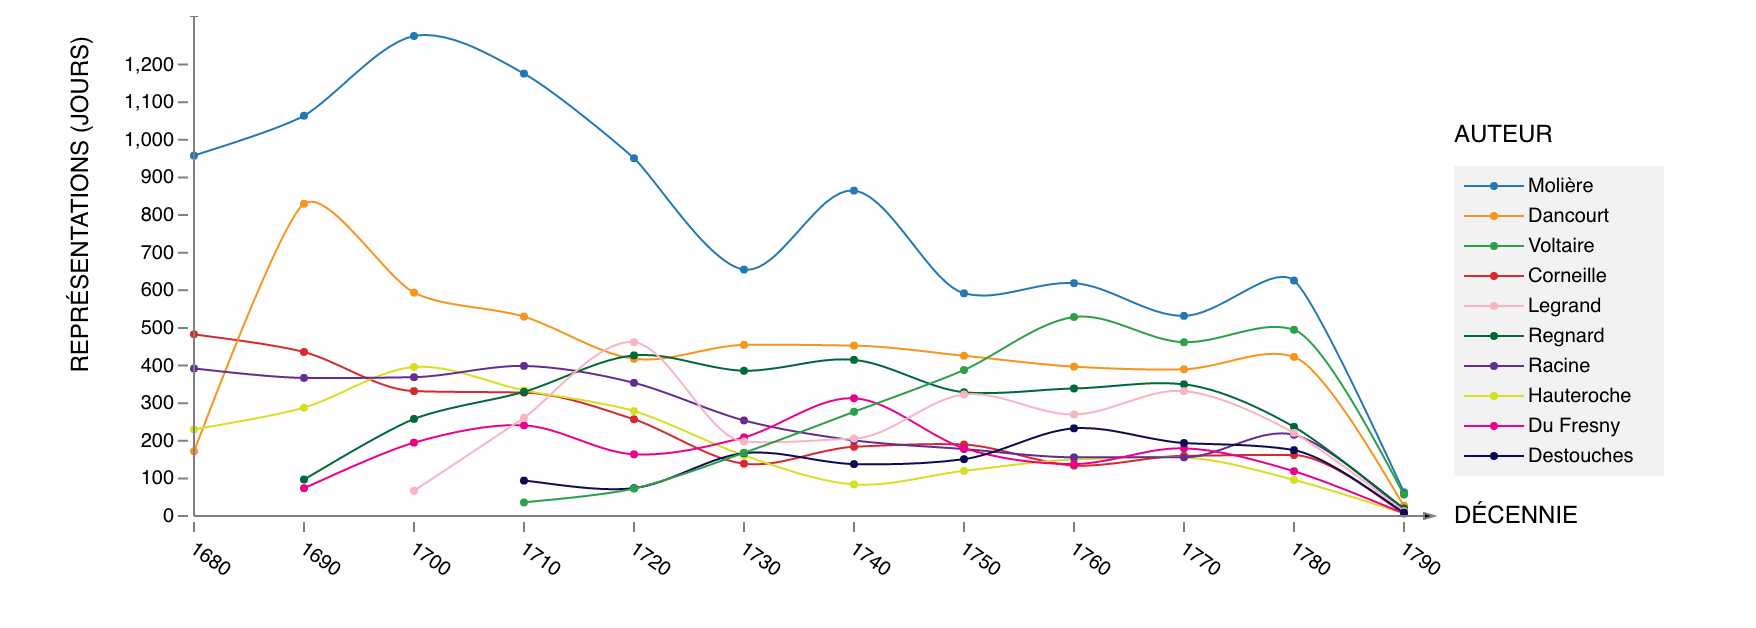
\includegraphics[width=7in]{steps/top-author-performances.png}
	\caption{Limiting the data graphed to the top or bottom ten lines (equivalent to sorting the CFRP crosstab table) allows users to clearly identify statistically-siginificant outliers, which are often more interesting than points close to the central tendency.}
	\label{fig:top-author-performances}
\end{figure*}

Thus far, most of the challenges our student faced while surveying the landscape of the Comédie Française database could be termed ``descriptive statistics'': identifying which are the relevant variables to explore, where the outlier datapoints lie and what the overall distribution of data suggests.  In addition to tackling these problems in research methodology, tools for working with digital humanities datasets must address the full spectrum of interpretive questions that lie at the core of traditional humanities practice.  For example, let us say our student, having explored some of the authorial patterns noted above, begins to wonder if the most-performed authors also constituted the bread-and-butter of the Comédie Française's box office takings.  Did the troupe use performances of plays by established authors to bankroll more speculative or ambitious plays by unknown authors?  Was there a particular season of the year, or day of the week that was particularly lucrative, and why?  Were some authors particularly lucrative, or particularly disastrous?

To dig into these questions, our student switches from looking at the number of performances by author, to gross ticket sales by author (figure \ref{fig:top-author-receipts}).  This graph tells a cautionary tale for the digital humanities, because it is so suggestive while being neither entirely compromised or self-evidently true.  Most strikingly, our student might note Voltaire's meteoric profitability after 1740 -- far out of proportion to the rise in his plays as a proportion of the number of performances by the Comédie Française troupe.  However, economic historians will already have sounded a note of caution: nominal livres earned in 1700 cannot be compared one-to-one to livres in 1760, as the value of the French currency fluctuated throughout time (as did the purchasing power of individual audience members).  So the student cannot conclude that Voltaire ``earned'' more for the Comédie Française in 1760 than Molière did in 1700-as the graph's scale cannot be compared horizontally-but she can still usefully note that there was a moment when Voltaire's plays became more lucrative than those of all other authors (because values \emph{can} be compared vertically, i.e. synchronically).

Armed with the historiographical knowledge that it is important to distinguish between nominal and real prices, our student can adjust the graph to show the latter. As figure \ref{fig:top-author-receipts-real} shows, after adjusting for inflation in the livre and yearly variations in the price of a ``basket of goods'', it appears that Voltaire's enormous profitability was a bona fide economic phenomenon.  Despite unrest and periodic agricultural failure throughout the 18th century, the Comédie Française took in increasingly more money in real terms in the years preceding the Revolution than it had in years immediately after it was founded.

\begin{figure*}
  \centering
	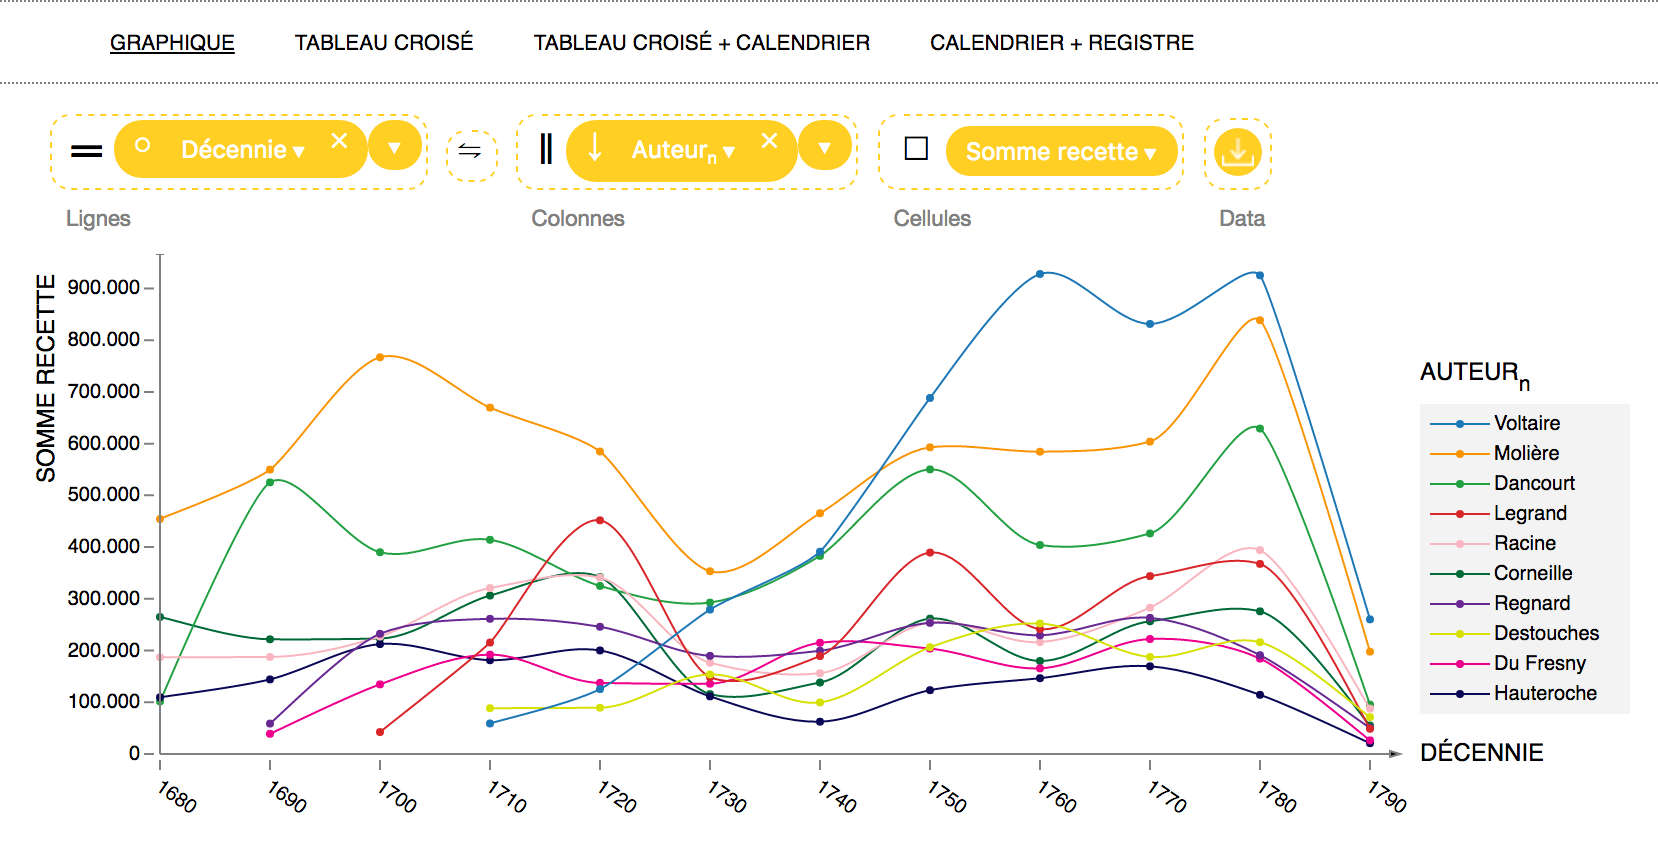
\includegraphics[width=7in]{steps/top-author-receipts-nominal.png}
	\caption{Nominal receipts aggregated by decade: the Comédie Française's most lucrative playwrights}
	\label{fig:top-author-receipts}
\end{figure*}

Digital tools and databases can be seductive and misleading, promising the possibility of immediate results and graphical answers to any question.  The example of nominal versus real prices above is crude but illustrative: how to slow users down so they properly consider source critique and look at archival materials before jumping to a conclusion based on the information in a single graph is an open problem.  To enumerate other examples immediately relevant to the Comédie Française project dataset:

\begin{description}
	\item[Double bills] Much as Golden Era Hollywood bundled two or more films together for sale in a single ticket, the Comédie Française rarely performed only a single play in an evening.  Instead theater-goers purchased entrance to an evening's entertainment, usually comprising a tragedy and a comedy, or two comedies (for example, 9 April 1723 saw a double bill of Molière's ``Tartoufe'' followed by his ``La Comtesse d'Escarbagnas''---see figure \ref{fig:register_example}).  Many intriguing research questions investigate which plays, authors or genres were performed on high- or low-grossing evenings.  Answering such questions properly is a problem in multivariate statistics, as both box office sales and the playbill varied each evening.  How do we convey this complexity to novice users of digital research tools - undergraduate students, for example - without oversimplifying the problem domain and implying a facile answer, or portraying it as hopelessly complex?

	\item[Changing seating areas] The Comédie Française itemized ticket sales by number sold in each seating area, which raises the inticing possibility of tracking how theater-goers from radically-different social strata consumed drama and engaged with radical new political philosophies.  But while the seating categories are available in the CFRP database, they changed frequently - sometimes in seeming contradiction to the physical layout of the Comédie Française's theater space.  The troupe also moved theaters four times between 1680-1793, making it very difficult to map audience demography onto the Comédie Française's archival record.  Indeed, it is even difficult to know how many people were in the audience, since loges seating 4-6 people were sold as a single ticket.  Without firm emphasis on primary source critique alongside digital tools to impress such considerations on students and other users, it would be easy to draw facile and baseless conclusions using data analysis tools: being able to work with data must go hand in hand with being able to \emph{critique} datasets.

	\item[Incomplete sources] Finally, the point that humanities datasets are rarely complete must be underlined.  While we can be reasonably sure the Comédie Française registers database maps all in-theater performances between 1680 and 1793, we also know that its ticket receipts comprise only a portion of the troupe's financial income.  Other, potentially large sums of money came into Comédie Française coffers as part of the royal pension and through aristocratic channels of patronage and gift.\cite{BROWN:2004}  Consequently, many of the assumptions of data science, which developed hand in hand with modern states and corporations who are reasonably sure of their own datasets, do not hold true for digital humanities databases.  Even after a thorough analysis of its ticket receipts, we cannot be sure the Comédie Française made institutional decisions based on profitability of plays.  Here again while the tools to do digital humanities analysis are sufficient and well-known, the materials with which digital humanists operate are fragmentary and suggestive rather than definitive.\todo{Check CF citation with Greg Brown.}

\end{description}

\begin{figure*}
  \centering
	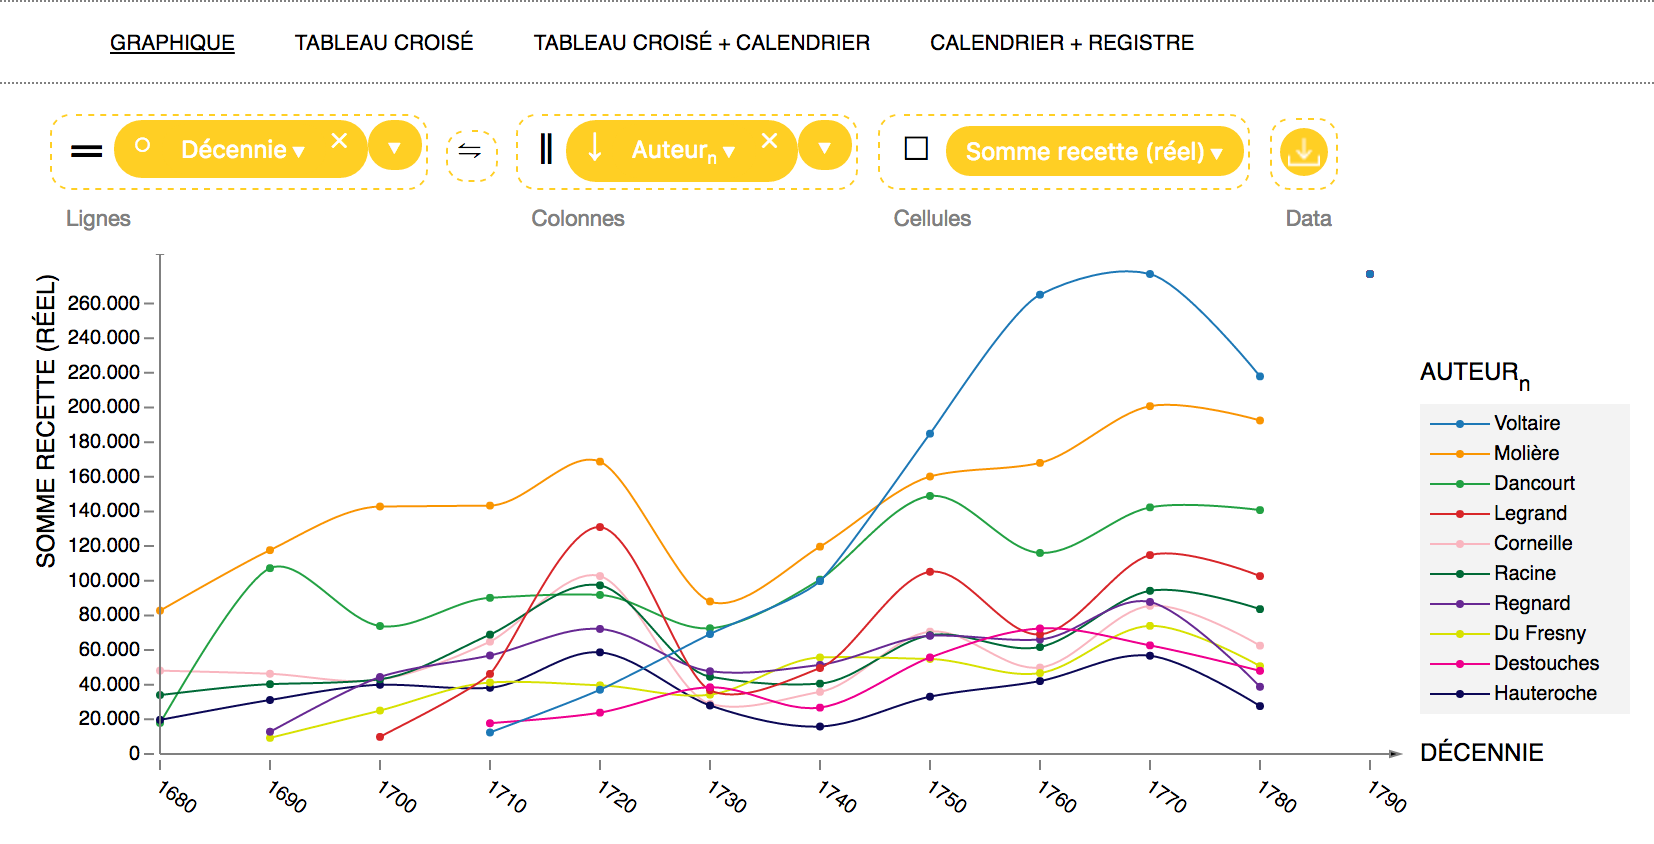
\includegraphics[width=7in]{steps/top-author-receipts-real.png}
	\caption{Real receipts (weighted by consumer price index)}
	\label{fig:top-author-receipts-real}
\end{figure*}

\subsection*{Drill-down: calendar}

In an article from 1996, ``The Eyes Have It,'' Ben Schneiderman introduced his influential visual information seeking mantra: ``Overview first, zoom and filter, then details on demand.''\cite{Shneiderman:1996}  The mantra identifies one successful narrative dynamic for information discovery in large datasets, in which the user first views an overview of the data ``landscape,'' then pursues phenomena of particular interest by zooming in on a regional sample or filtering the entire dataset using search criteria.  At this point the user is likely to want to confirm individual data points by clicking to bring up ``details on demand.''  From here, the process loops back iteratively as necessary to examine other slices of the data landscape that support or disprove the insight being exploring, but using other data points.

Certainly Scheiderman’s mantra applies to general-purpose use of CFRP’s Crosstab table, as users select data categories, filter or scroll down to particular columns or rows of interest, and mouse over individual table cells to see details of a particular aggregate.  However, the CFRP Crosstab tool was designed to support Schneiderman’s information seeking mantra in a fashion shaped by the particular concerns of humanities research.

The CFRP Crosstab’s calendar function leverages characteristic feature of the Comédie Française registers: with only one performance session per day, the Comédie Française dataset can be arranged to expose the one-to-one correspondence between dates and archival pages.  So, on switching from the table view to the calendar (see figure \ref{fig:calendar-receipts}), one sees the same data aggregation, but mapped in quantiles by day.  From here one can zoom in on a specific range of days by highlighting them.

\begin{figure}
  \centering
	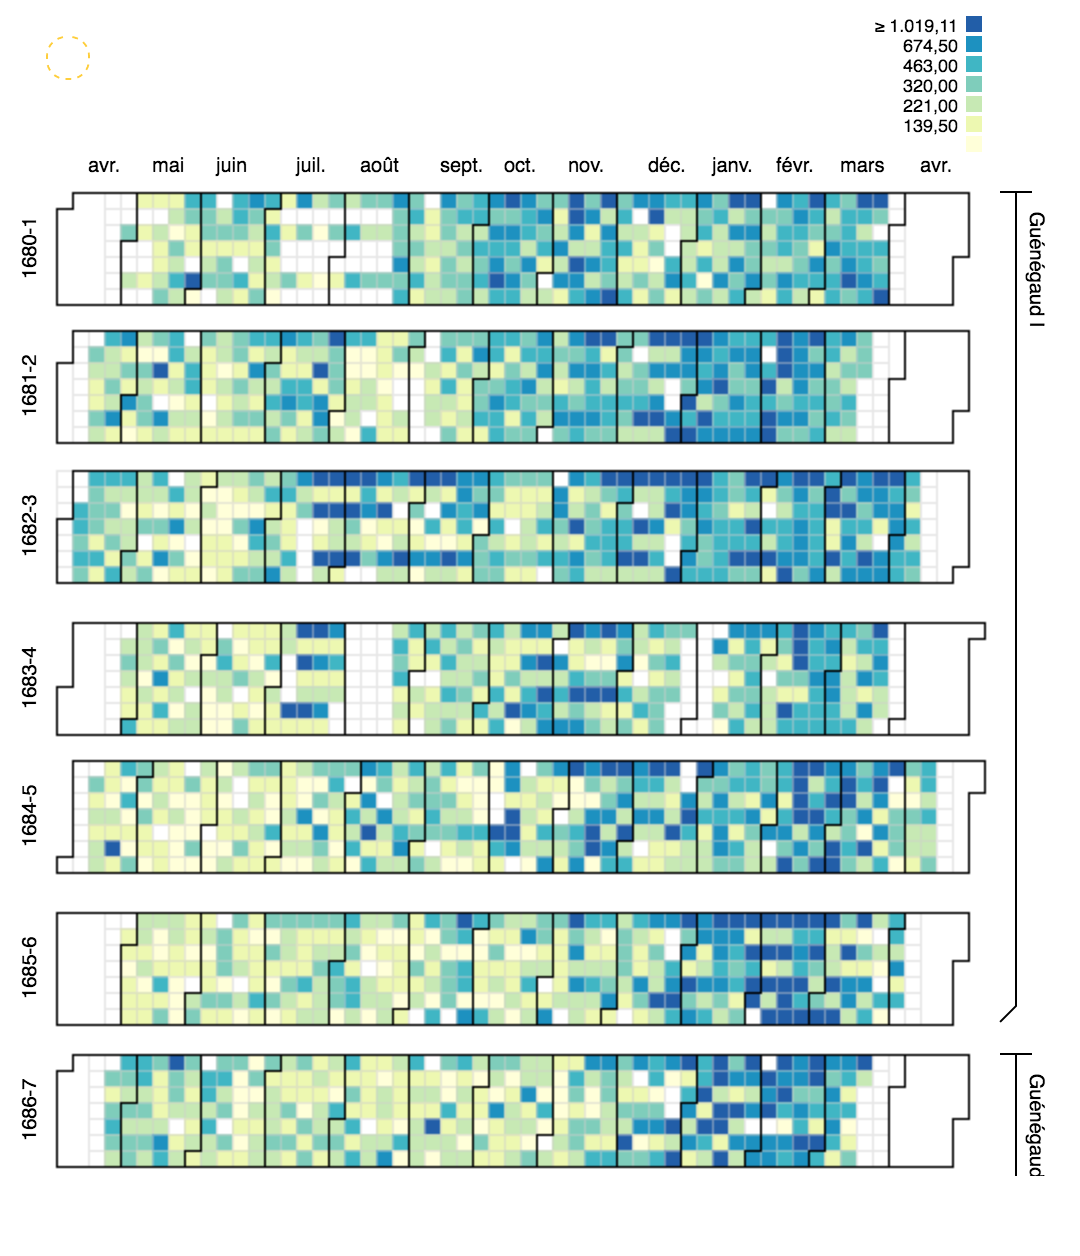
\includegraphics[width=3.25in]{steps/calendar-receipts.png}
	\caption{Daily receipts: All evenings}
	\label{fig:calendar-receipts}
\end{figure}

By arranging statistics in a visual that emphasizes cycles over time, the calendar was designed to explore the middle ground between free-form data analysis and a purpose-crafted visualisation.  On switching to it, our student is likely to notice patterns that disappear when data is aggregated at a higher level.  The Comédie Française season ran from Easter to Easter, moving every year with the Church's calendar, so the tool accommodates this by plotting 13 months with April duplicated on left and right margins.  Our student can trace patterns in high-grossing ticket sales vertically across months or horizontally across days of the week.  (She might immediately note a seasonal swing between summer months when the troupe took a moderate but steady profit, compared to the dark blue winter productions, when profits rose as military conscripts came home from their service.)

Weekly variations in the Comédie Française's programming appear here as well: for example, the pattern of high-grossing runs on Sundays, Tuesdays and Fridays as seen in July of the 1683-4 season.  By clicking on the calendar, our student can drill down to digital images of the Comédie Française registers for these particular days, finding that these corresponded to a particularly successful run of Corneille's tragedy ``La Toison d'or''; or use the tools to limit entries visualised in the calendar to plays by Corneille only (see figure \ref{fig:register-image-corneille}).

\begin{figure*}
  \centering
	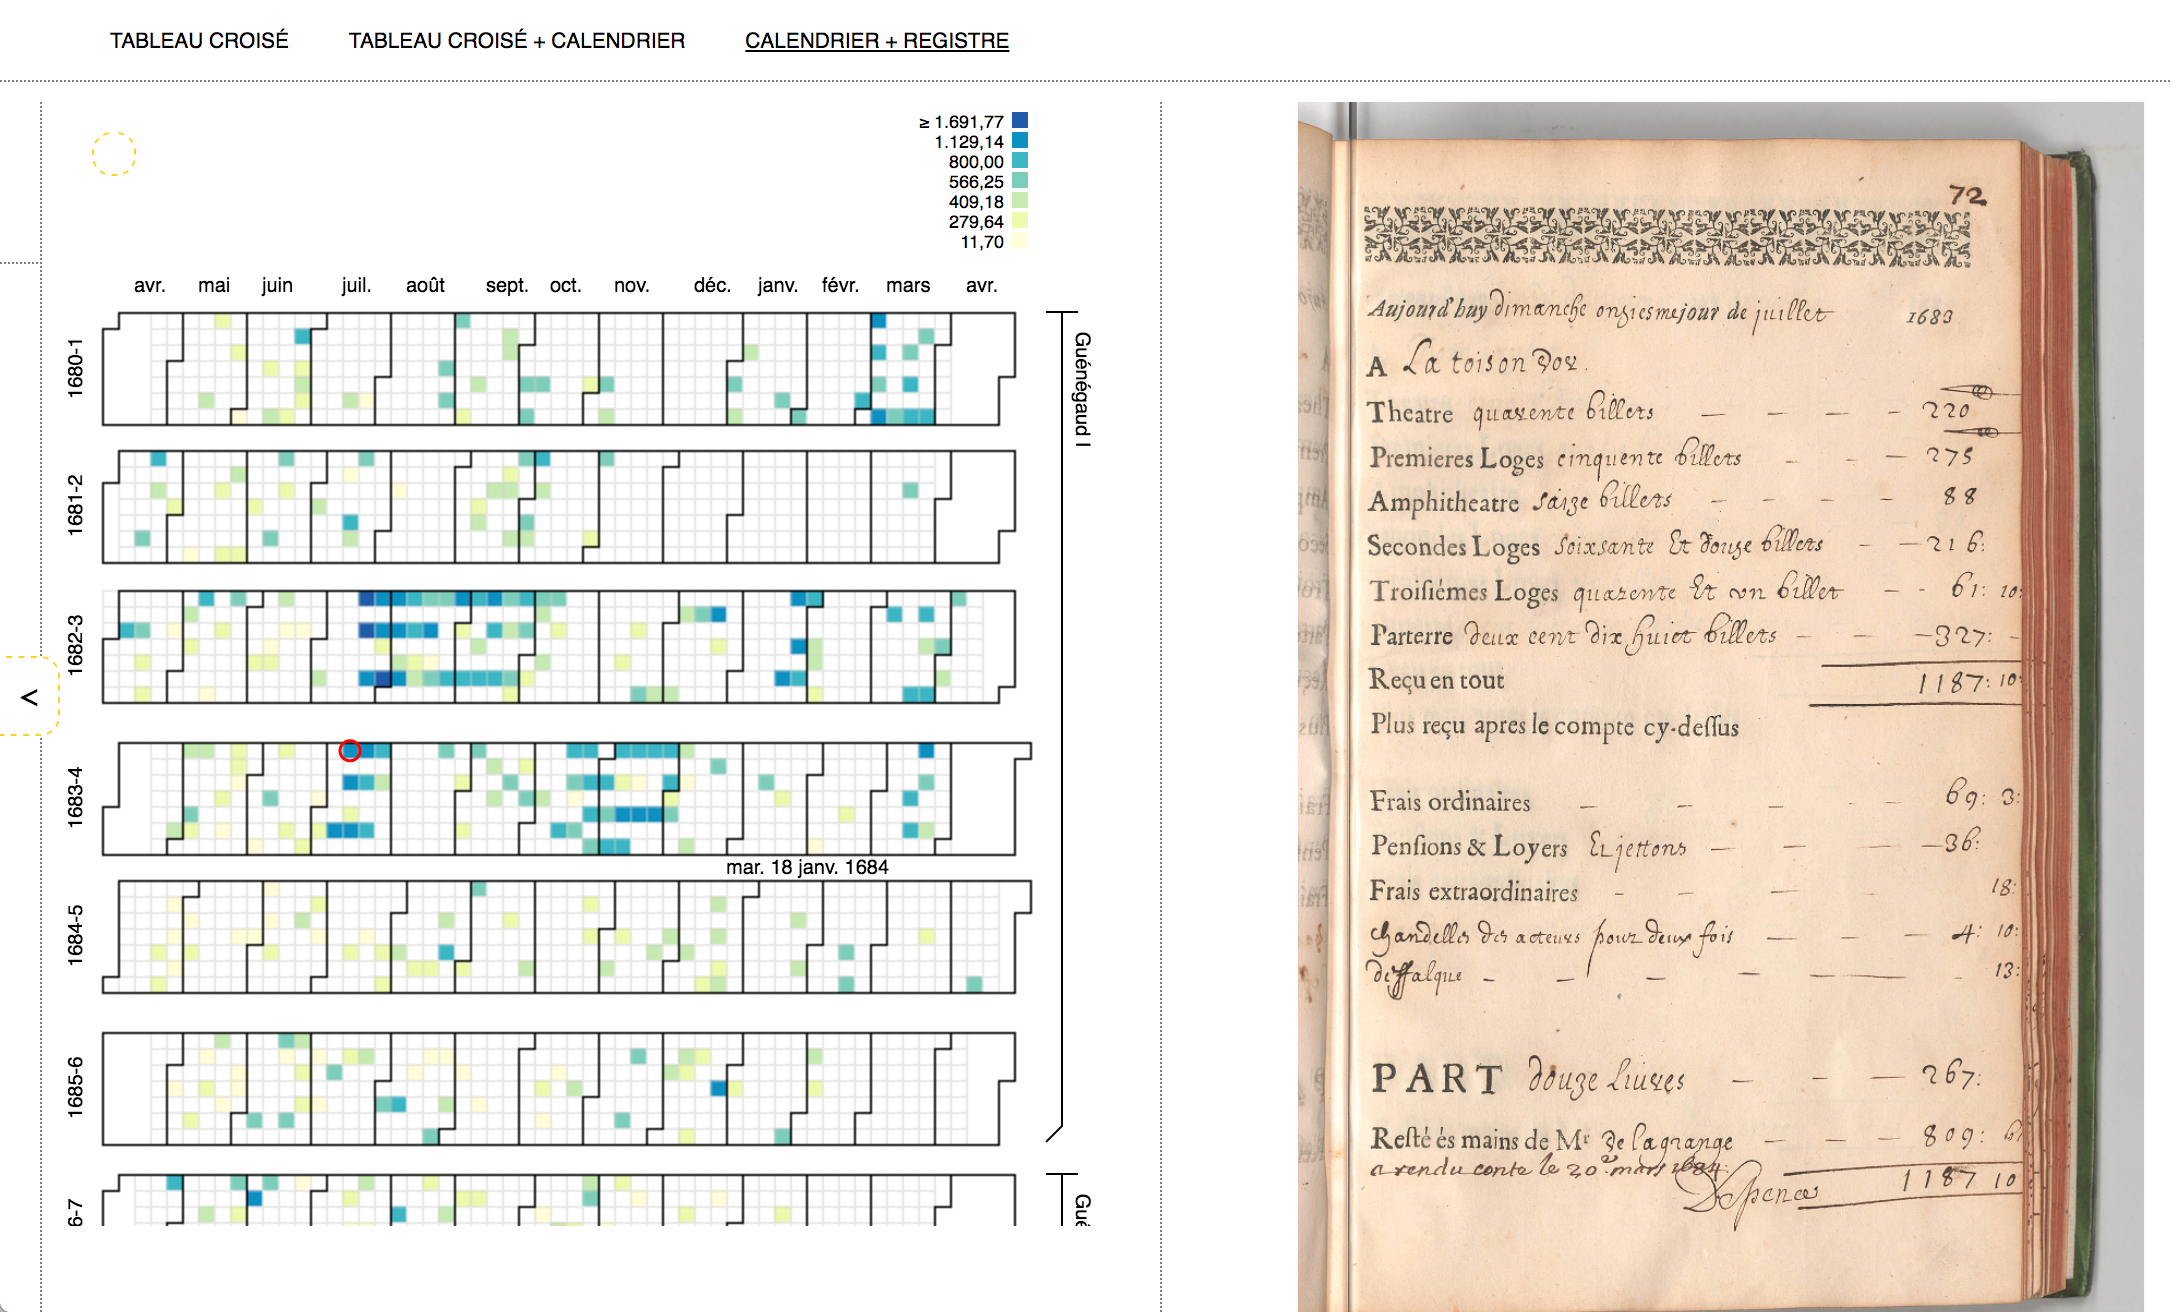
\includegraphics[width=7in]{steps/register-image-corneille.png}
	\caption{Daily receipts: Evenings when a play by Corneille was performed, e.g. ``La Toison d'or''}
	\label{fig:register-image-corneille}
\end{figure*}

The CFRP filter and refinement tools apply to the calendar, just as they did to the Crosstab Table.  For example, after looking at ``La Toison d'or'', our student might wonder if the Comédie Française programmed tragedies like Corneille's on particular week-nights.  She de-selects Corneille and instead configures the Crosstab Table to show ticket receipts summed by play genre, then limits to only comedies and tragedies.  With the Crosstab Table and calendar side by side, she can click on individual cells in the table to visualise the results in the calendar.  Viewing the pattern of comedies and tragedies in turn (figures \ref{fig:comedies-calendar} and \ref{fig:tragedies-calendar}) for example, she might begin to see the outlines of a weekly pattern for the Comédie Française, of opening Sundays, Tuesdays and Fridays with a comedy followed by a high-earning tragedy, with Mondays Wednesdays and Saturdays reserved for lighter, more comedic fare throughout.

\begin{figure*}
  \centering
	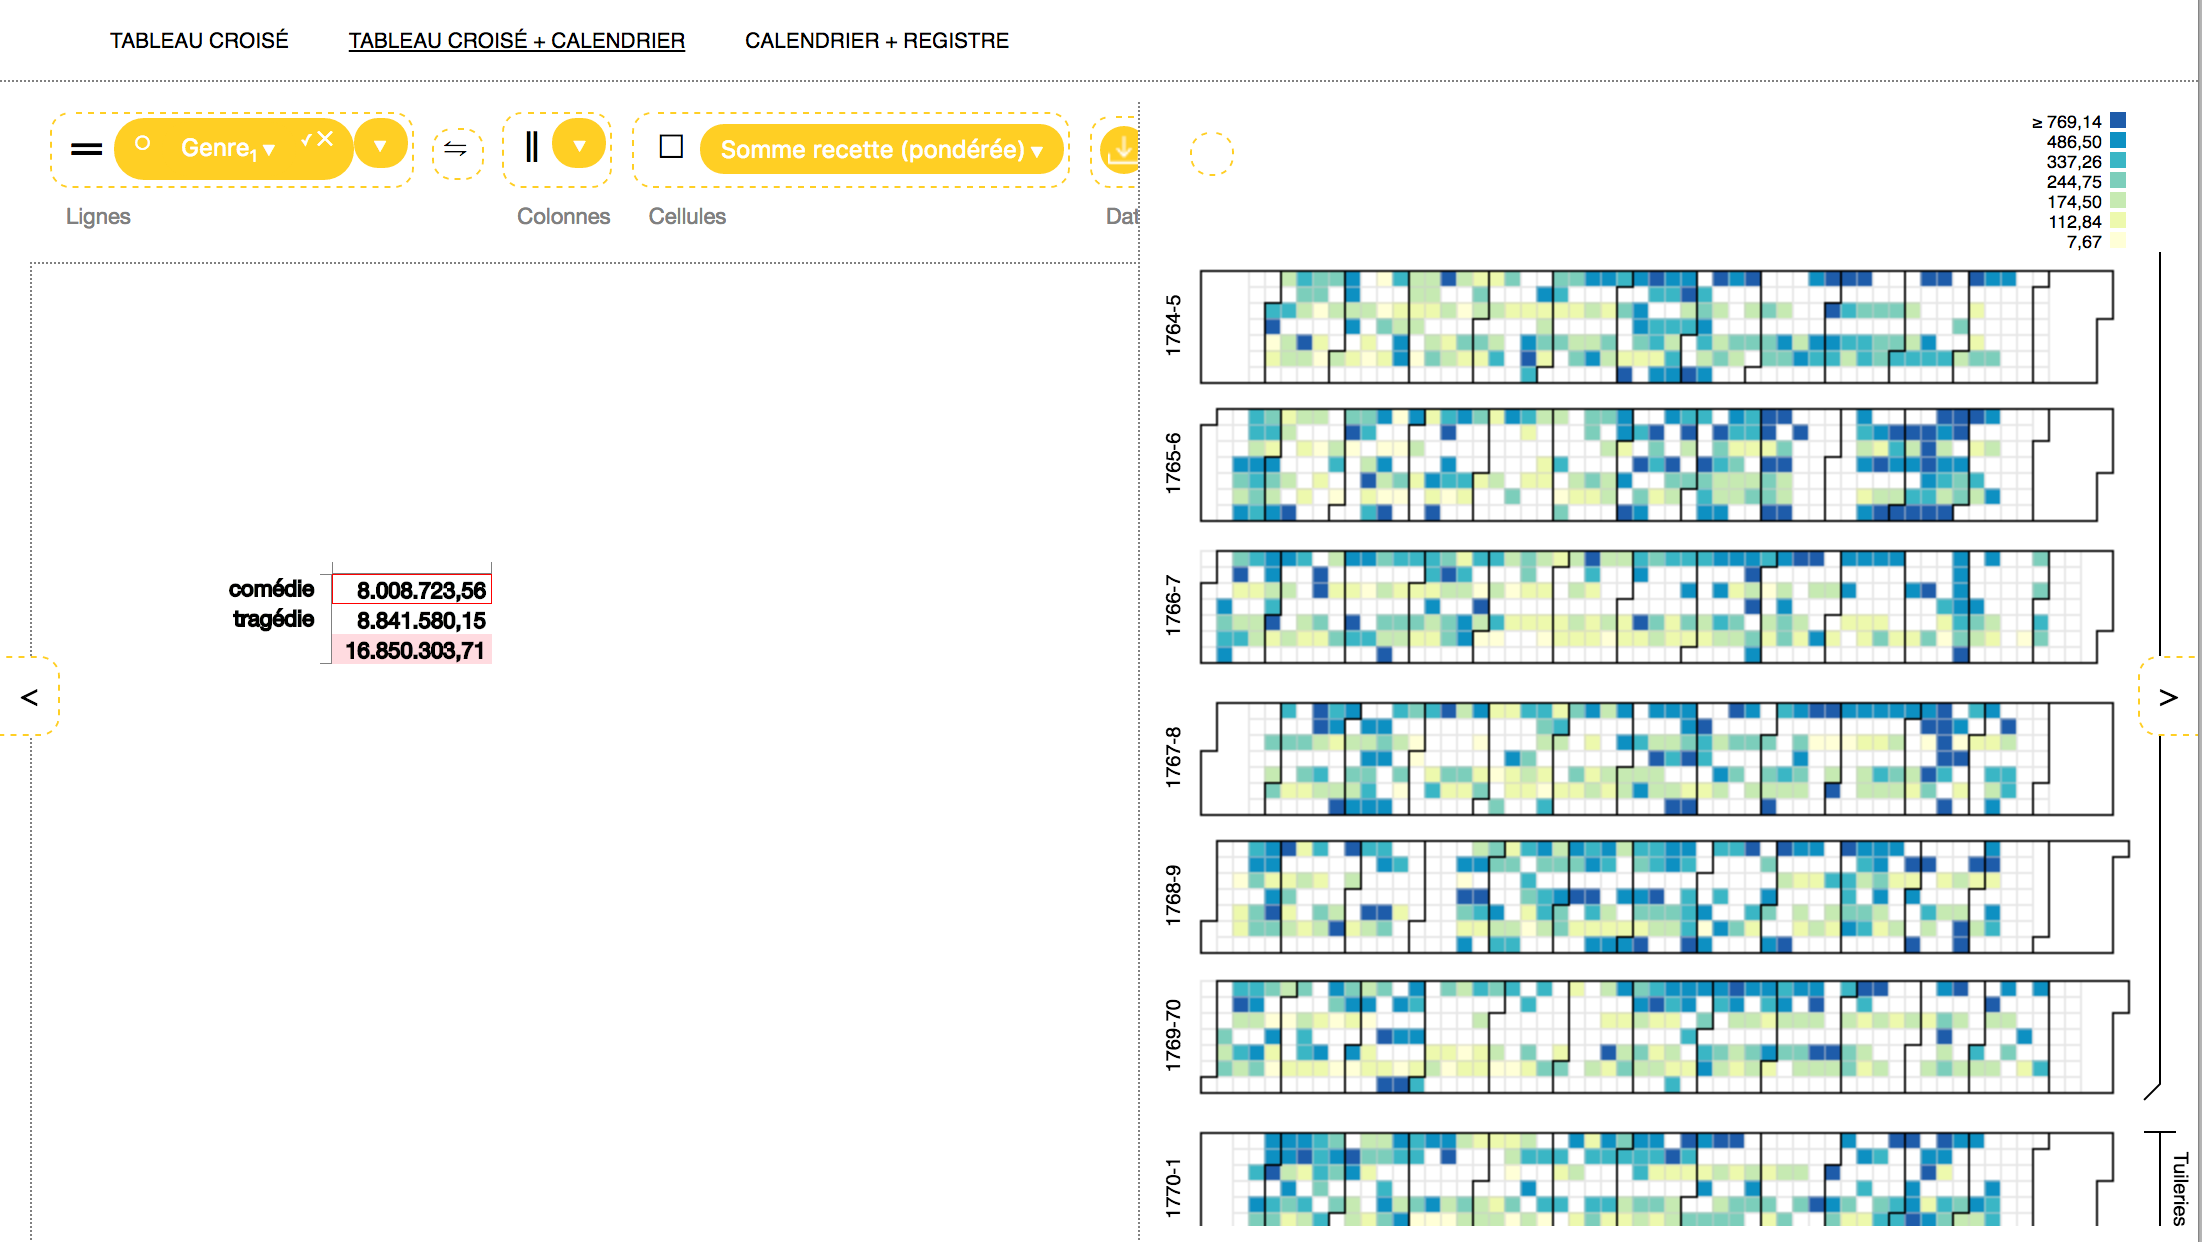
\includegraphics[width=7in]{steps/comedies-calendar.png}
	\caption{Drilling down to a specific table cell: calendar of ticket receipts when a comedy opened the night}
	\label{fig:comedies-calendar}
\end{figure*}

\begin{figure*}
  \centering
	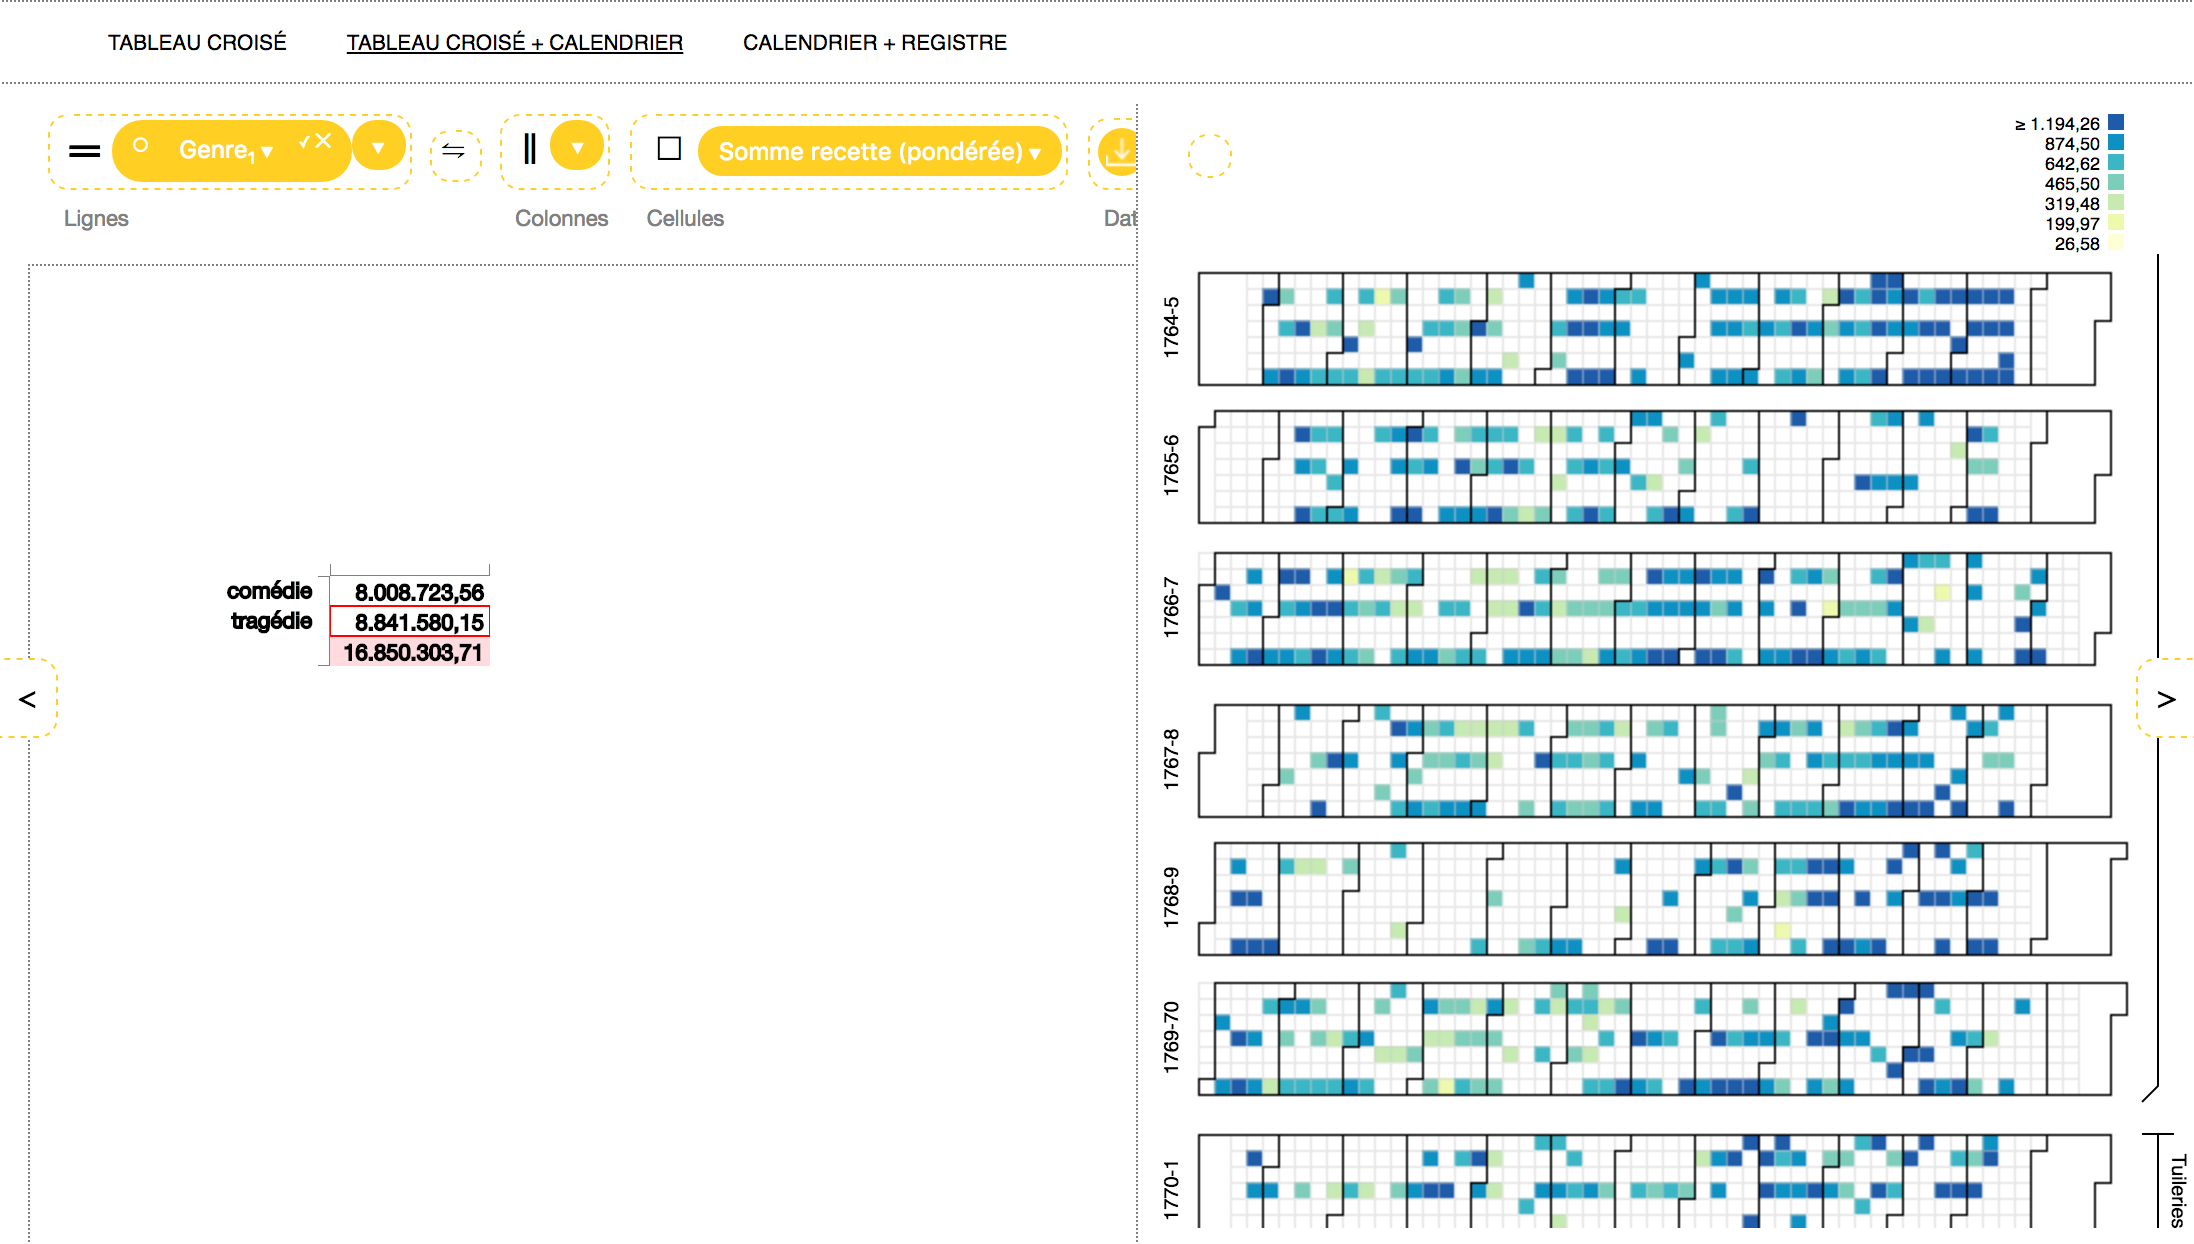
\includegraphics[width=7in]{steps/tragedies-calendar.png}
	\caption{Drilling down to a specific table cell: calendar of ticket receipts when a tragedy opened the night}
	\label{fig:tragedies-calendar}
\end{figure*}

More importantly, however, from here the ``details on demand'' pull up individual archival pages for the performance session on a given day.  This allows the user to confirm computer analyses by direct inspection of archival sources...

\section*{Conclusion}

My aims in this paper have been as follows.

First, to describe the workings of a generalist suite of open-ended tools for analyzing humanities data sets associated with an important historical literary institution.  I described the rationale for including the specific tools in our project, and walked through several characteristic paths an undergraduate student might take as she first surveyed the landscape, then drilled deeply into a particular vein of data.

A repeated theme along the way has been the tension between tools that enable users to answer a particular question using \textbf{data analysis} - ``did Voltaire's comedies or his tragedies gross more in the 1760s?'' - versus those that enable \textbf{data analytics} - ``what are notable features relating to play genre?''  In the former case, the subject expert uses digital research tools to gather evidence relating to a specific question in a known field of enquiry: the domain is known beforehand, and the resulting visualisation marshals visual evidence rhetorically to prove the author's point.  By contrast, in the latter case a subject neophyte uses digital tools to discover first features of an unknown field of enquiry: not, ``what is the answer to this question?'' but rather ``what are the meaningful questions to ask?''.  The visualisations deployed in this quest are necessarily general-purpose - simple bar, line and scatter charts.  Uncharted caves are explored using a simple headlamp; only once we discover Lascaux do we bring in the laser show to convince others of the importance of what we have found.  Where an individual digital humanities tool or visualisation lies on this spectrum is an important question to answer.

Second, to make a case for introducing data literacy, and experimentation with tools like these, into undergraduate education in the humanities.

(2.1) Data literacy: humanities education places a strong emphasis on developing student skills in critiquing primary sources and examining evidence marshalled by others to support a historical or literary argument.  At first exposure the tools, techniques and concerns of data science and database analysis seem foreign to the humanities, but they can be taught and learned as a stepwise extension of traditional scholarly scepticism, moving from qualitative sources of evidence to quantitative ones.  Data literacy - in the form of fluency with descriptive statistics - often suffices to make nuanced arguments about humanities datasets derived from cultural heritage sources.  Witness, for example our opening observation in figure \ref{fig:tukey_boxplot} about median performance statistics: that 50\% of Comédie Française authors were performed fewer than 17 evenings.  This merely formalises an insight that archival historians might previously have summarised as, ``examination of the daily registers reveals the extent to which Molière, Racine and Corneille dominated the Comédie Française repertory.''  Rising data literacy will enable humanists to walk easily between two such idiomatic formulations, and see them as expressions of similar insights.

As students' data literacy rises, we can expect to see an increasingly nuanced vocabulary for critiquing digital humanities visualisations develop in parallel.  For example, examining visualisations through the lens of Tukey's distinction between exploratory and confirmatory data analysis allows us to pierce through a fascination with "pretty pictures" to identify visuals that suggest the outlines of a hidden data landscape; or to examine how the author marshals visual marks as a rhetorical argument, just as humanities scholars have done in text for centuries.

At the same time, it is worth emphasizing areas in which digital humanities datasets and methods necessarily differ from those of the natural and social sciences, rendering them only partially compatible to existing data analysis tools.  Humanities evidence is necessarily partial, contingent and suggestive, arriving as it does mediated by institutional and state archives, depleted by accidental or polemic elisions by any one of a number of historical actors.  Connoisseurship, close-reading and interpretation plays a correspondingly larger role in disciplines that are data-poor and rich in meaning.  One way to keep this methodological scepticism alive for students to balance and link ``digested'' digital humanities datasets to the ``undigested'' archival images they were derived from, and to encourage students to move between the two regularly to confirm and critique the conclusions of data analysis by reference to primary sources.

(2.2) The pedagogical importance of playing with tools: the critical-information scholar Mark Ratto uses the term "critical making" the describe the ability of hands-on design practice to produce distinctive kinds of knowledge.  In the examples used here, we presented students with a historical institution (the Comédie Française) as an occasion, not merely for analysis, but for working through a problem via methods that aim to produce, even speculatively, a tool, a procedure, an artifact.  It is possible to discuss the history of the Comédie Française simply by way of assigning and discussing articles and book chapters--indeed, it is easier that way.  Discussing this history as a problem in data analysis creates an obstacle--a productive constraint--that may help us to produce new concepts or to think through old concepts in new ways.

Third, I hope that this essay will encourage humanists who specialize in traditional methods of analysis to expand their repertoires to work on projects of this kind.  The humanities have much to contribute to the kind of world-building that computer science, in its push to develop tools and systems for managing information, has obsessively engaged in.  Our intellectual inheritance includes forms of theoretical and methodological expertise - the scholarly inheritance of a data-poor but meaning-rich materials - on which present computational methods have little purchase.  As we continue to engage with new waves of scholarship that bring new computational tools to the humanities, we will need to keep finding ways to balance digital methods with ``digital critique'': the computational analogue to our methodological scepticism, literary sensibility and temperamental openness to human experience and openness to interpretation and polysemy.  This will only happen if traditional humanists continue to work with data scientists, just as traditional humanists and critical-information experts worked together on this project.  I hope that the achievements and possibilities of the Comédie Française Registers Project will spur others to creative experimentation.

\printbibliography

\end{document}
